\documentclass[uplatex, dvipdfmx, a4paper, report, papersize, 11pt]{jsbook}
\usepackage{bm}
\usepackage{amsmath}
\usepackage[dvipdfmx]{graphicx}
\usepackage{wrapfig}
\usepackage[hang, small, bf]{caption}
\usepackage[subrefformat=parens]{subcaption}
\usepackage{comment}
\captionsetup{compatibility=false}

\bibliographystyle{jplain}
\title{二色の光周波数コムによるレーザー冷却法の開拓}
\author{物理工学科4年 中西亮}
\date{2018/11/19}
\begin{document}
\maketitle
\newpage

\setcounter{tocdepth}{2}
\tableofcontents

\newpage
\chapter{過去の研究}
\section{従来の課題と光周波数コムによる冷却のメリット}

 従来のレーザー冷却では, アルカリ金属やアルカリ土類金属などの限られた原子しか冷却できなかった.この理由としては主に2つの理由が挙げられる. 1つ目としては, 水素や酸素を含む多くの原子の遷移エネルギーは真空紫外領域に相当しており現在はこの領域で十分な強度のレーザーを得ることができていないことがある. 2つ目は, 多くの原子ではエネルギー準位の構造が複雑であり励起された原子が準安定な準位に緩和してしまうので, これを励起するためのレーザーを用意する必要があり実験の系が複雑化してしまうことである\cite{PhysRevA.73.063407}.\\
 光周波数コムを用いた二光子のレーザー冷却は, 2006年にKielpinski\cite{PhysRevA.73.063407}によって提案された. 光周波数コムを用いることにより, 上記の2つの課題を克服することができる. まず, 光周波数コムは高強度のピークパワーをもつため, 同じ時間平均パワーをもつcwレーザーに比べて高効率の非線形工学効果を利用することができ, より高強度の短波長のレーザーを得ることができる. また, 光周波数コムの一つ一つのの縦モードがリポンプレーザーとして機能するために, 実験の系を簡単にすることができる. これらの長所により, 光周波数コムはcwレーザーよりも効率の良い二光子冷却を実現することができる\cite{PhysRevA.73.063407}.\\
 本章では, コムを用いた二光子冷却についての過去の研究の内容を紹介する.

\section{二光子コムによるレーザー冷却の理論}
 Jayichらの論文\cite{PhysRevX.6.041004}で説明されている, 二光子遷移を用いたレーザー冷却の理論を紹介する.\\
コムによる二光子の遷移を考えるとき, パルスに含まれる二光子のエネルギーもまた, コム(櫛)を形成する.これを二光子コムと呼ぶことにすると, 二光子コムのn番目の縦モードの周波数は
\begin{equation}
f_n = nf_r + 2f_0
\end{equation}
となる. ただし, $f_r$:は繰り返し周波数, $f_0$はキャリアエンベロープオフセット周波数を表す.チャープのモード同期レーザーについては実効的な共鳴ラビ周波数を求めることができる. 二光子コムのn番目のコムの歯共鳴ラビ周波数は,
\begin{eqnarray}\label{ResonanceRabi}
\Omega _{n} &=&\sum _{p}\frac {g^{\left( 1\right) }_{p}g^{\left( 2\right) }_{n-p}}{2\Delta_p} \nonumber\\
&=& \sum _ { p } \frac { e ^ { 2 } \mathcal { E } _ { p } \mathcal { E } _ { n - p } } { \hbar ^ { 2 } } \left\langle \mathrm { e } \left| ( \hat { \boldsymbol { \epsilon } } \cdot \mathbf { r } ) \left( \sum _ { \mathrm { i } } \frac { | \mathrm { i } \rangle \langle \mathrm { i } | } { 2 \Delta _ { p } ^ { ( \mathrm { i } ) } } \right) ( \hat { \boldsymbol { \epsilon } } \cdot \mathbf { r } ) \right| \mathrm { g } \right\rangle
\end{eqnarray}\\
ただし, $g^{\left( 1\right) }_{p}$は$p$番目のコムの歯による基底状態から中間状態への共鳴一光子ラビ周波数, $g^{\left( 2\right) }_{p}$は$p$番目のコムの歯による中間状態から励起状態への共鳴一光子ラビ周波数を表す.
$\Delta _{p}=pf_{r}+f_{0}-f_{gi}$は一光子の中間状態からの離調である. ただし, $f_{gi}$は基底状態から中間状態へのエネルギー差をプランク定数$h$で割ったものである.また、$\epsilon_0$は真空の誘電率、$c$は光速、$e$は電気素量、$\hbar$はプランク定数$h$を$2\pi$で割った値を表す。\\
二光子コムのN番目のコムの歯が共鳴周波数に最も近いとき, 速度$v$で動く原子の励起確率の時間平均は,
\begin{equation}\label{ExcitationRate}
\gamma_\mathrm{comb} = \frac{\Omega^2_{N}T_\mathrm{r}} {4} \frac{\sinh(\gamma T_\mathrm{r}/2)}{\cosh(\gamma T_\mathrm{r}/2) - \cos(\delta_N(\bm{v})T_\mathrm{r})}
\end{equation}
ここで, $\delta _{N}\left( v\right) \equiv 2\pi ( f_\mathrm{\mu }-f_\mathrm{ge}-f_{N}\widehat {\bm{k}}\cdot {\bm{v}}/c )$は$N$番目の二光子コムの歯の共鳴周波数からの離調を表す.$f_{ge}$は励起状態と基底状態のエネルギー差をプランク定数で割ったもの, $\widehat {\bm{k}}$はレーザーの進行方向の単位ベクトル, $\gamma$は励起準位の自然幅を表す.\\
離調$\delta _{N}\left( v\right)$と自然幅$\gamma$の両方がコムの歯の間隔($2\pi f_r$)よりも小さいとき, 二光子コムは二光子ラビ周波数$\Omega_N$の一つの縦モードとして扱うことができる.この近似の下では, 励起確率は
\begin{equation}\label{EffectiveExcitationRate}
\gamma_N = \frac{\Omega^2_N}{\gamma}\frac{1}{1 + [2\delta_N(\bm{v})/\gamma]^2}
\end{equation}
と表せる.\\
 また, (二色のコムによる冷却ではなく)縮退したコムによる二光子冷却の場合, ドップラー冷却限界温度は
\begin{equation}
  T_\mathrm{D} = \frac{3}{4}\frac{\hbar\gamma}{2k_\mathrm{B}}
\end{equation}
となることが分かっている. ただし, $k_\mathrm{B}$はボルツマン定数\\
 Jayichらの論文\cite{PhysRevX.6.041004}では, 初めて光周波数コムを用いた二光子冷却の実証実験が行われた.Jayichらのグループはルビジウムの縮退した二光子のコムによる一次元のレーザー冷却に成功し, 57 $\mu$Kを達成している.

\section{Cs原子の二色のコムによる励起効率の見積もり}
 Jayichらの論文\cite{PhysRevX.6.041004}では、5s軌道から5d軌道への遷移を利用しており、以下のパラメータの下で実験を行っている。
\begin{itemize}
  \item 5d順位の線幅 : $2\pi \times 667$ kHz
  \item レーザーのパルス幅 : $2-5$ ps
  \item レーザーのパワー : $500$ mW
  \item レーザービームの直径 : $1$ mm
  \item レーザーの周波数幅 : $500$ GHz
  \item コムの繰り返し周波数 : $80$ MHz
\end{itemize}
Jayichらはこのパラメータの下で励起効率を$\gamma_N \sim 13000\ \mathrm{s^{-1}}$と見積もっている。\\
 Jayichらの論文\cite{PhysRevX.6.041004}の励起確率の計算手法に習い、今回私達の用いるコムでCs原子を冷却する際の励起確率の計算を行った。その計算に際して以下の五つの近似を行った。\\
\\
 (a) $\delta_N(\bm{v}) = 0$とし、
\begin{equation}
  \gamma_N = \frac{\Omega^2_N}{\gamma}
\end{equation}
     とした。\\
 (b) 二光子励起の際の中間状態として$6P_{\frac{3}{2}}$以外の状態を無視した。\\
 (c) 光周波数コムの全ての縦モードの電場の強さが一定であるとして計算を行った。
\begin{equation}
  \mathcal{E}_p = const.
\end{equation}
 (d) 以下の関係式を用いた。
\begin{equation}
  \Sigma_{p} \mathcal{E}_p\mathcal{E}_{n-p} \approx 2I/\epsilon_0 c
\end{equation}
 (e) $\left\langle \mathrm { e } \left| ( \hat { \boldsymbol { \epsilon } } \cdot \mathbf { r } ) | \mathrm { i } \rangle \langle \mathrm { i } |  ( \hat { \boldsymbol { \epsilon } } \cdot \mathbf { r } ) \right| \mathrm { g } \right\rangle$ の値がCs原子とRb原子で等しいとした。\\
\\
 (a)-(d)の近似を用いると、励起効率の式(\ref{EffectiveExcitationRate})は以下のように計算できる。\\
\begin{eqnarray}
  \gamma_N &=& \frac{\Omega^2_N}{\gamma}\frac{1}{1 + [2\delta_N(\bm{v})/\gamma]^2} \nonumber\\
  &=& \frac{\Omega^2_N}{\gamma}  \nonumber\\
  &=& \frac{1}{\gamma} \Biggl[ \sum _ { p } \frac { e ^ { 2 } \mathcal { E } ^{(1)}_ { p } \mathcal { E }^{(2)} _ { N - p } } { \hbar ^ { 2 } } \left\langle \mathrm { e } \left| ( \hat { \boldsymbol { \epsilon } } \cdot \mathbf { r } ) \left(  \frac { | \mathrm { i } \rangle \langle \mathrm { i } | } { 2 \Delta _ { p } ^ { ( \mathrm { i } ) } } \right) ( \hat { \boldsymbol { \epsilon } } \cdot \mathbf { r } ) \right| \mathrm { g } \right\rangle \Biggr]^2 \nonumber \\
  &=& \frac{1}{\gamma} \Biggl[ \sum _ { p } \frac { e ^ { 2 } \mathcal { E }^{(1)} \mathcal { E } ^ {(2)} } { \hbar ^ { 2 } } \left\langle \mathrm { e } \left| ( \hat { \boldsymbol { \epsilon } } \cdot \mathbf { r } ) \left(  \frac { | \mathrm { i } \rangle \langle \mathrm { i } | } { 2 \Delta _ { p } ^ { ( \mathrm { i } ) } } \right) ( \hat { \boldsymbol { \epsilon } } \cdot \mathbf { r } ) \right| \mathrm { g } \right\rangle \Biggr]^2 \nonumber \\
  &=& \frac{e^2  \mathcal { E } ^ {(1)} \mathcal { E } ^ {(2)}}{ 2 \gamma \hbar ^ { 2 }  }\Biggl[ \left\langle \mathrm { e } \left| ( \hat { \boldsymbol { \epsilon } } \cdot \mathbf { r } ) | \mathrm { i } \rangle \langle \mathrm { i } |  ( \hat { \boldsymbol { \epsilon } } \cdot \mathbf { r } ) \right| \mathrm { g } \right\rangle\sum _ { p }\frac{1}{2 \Delta _ { p } ^ { ( \mathrm { i } ) }} \Biggr]^2\\
  \mathcal{E}^{(i)} &=&  \sqrt{\frac{2 I_{i}}{M \epsilon_0 c}}\ \ \ \ (i = 1,2)
\end{eqnarray}\\
ただし、$\mathcal{E}^(1)_p$は基底状態から中間状態へのコムの$p$番目の縦モードの電場の大きさを表し、、$\mathcal{E}^(2)_p$は中間状態から励起状態へのコムの$p$番目の縦モードの電場の大きさを表す。$\mathcal{E}^{(i)}\ \ (i = 1,2)$は近似(c)の下でのコムの電場の強さを表す。$I_{i}\ \ (i = 1,2)$はそれぞれのコムの強度を表す。$M$はコムの歯の本数を表し、計算上では2つのコムの歯の数は等しいとした。\\
 まず、Jayichらのグループが計算で得た励起効率から計算すると
\begin{equation}
\left\langle \mathrm { e } \left| ( \hat { \boldsymbol { \epsilon } } \cdot \mathbf { r } ) | \mathrm { i } \rangle \langle \mathrm { i } |  ( \hat { \boldsymbol { \epsilon } } \cdot \mathbf { r } ) \right| \mathrm { g } \right\rangle = 4.1 \times 10^{-22}
\end{equation}
を得る。この値をCsでも用いて計算する。\\
 実験系の以下のパラメータを用いて二色のコムでの励起効率の計算を行った。
\begin{itemize}
  \item 遷移 : 6sから8s
  \item 5d順位の線幅 : $2\pi \times 2.18$ MHz
  \item レーザービームの直径 : $0.5$ mm
  \item 760nm付近の波長を持つコムの強度 : $1$ W
  \item 894nm付近の波長を持つコムの強度 : $10$ mW
  \item コムの繰り返し周波数 : $1.6$ GHz
  \item 中間状態にもっとも近い二光子コムの歯の$6P_{\frac{3}{2}}$からの離調が$2 \mathrm{GHz}$
\end{itemize}
 この条件で一光子コムの周波数幅を変化させて励起効率を計算すると、図\ref{2color_excitation_rate}のようになった。切り出す周波数幅を大きくすると、中間状態からの離調が大きくなる分、励起効率が落ちることがわかる。ただし、切り出す周波数幅を小さくするとコムの強度も落ちるが、この効果は計算に取り入れられていない。

\begin{figure}[htbp]
 \begin{center}
  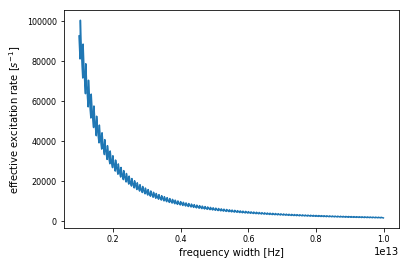
\includegraphics[width=100mm]{figures/chapter3/2color_excitation_rate_astro.png}
\end{center}
 \caption{二光子励起効率の一光子コムの周波数幅に対する依存性}
 \label{2color_excitation_rate}
\end{figure}

\chapter{Cs原子のMOTのためのcw光源の構築}
\section{飽和吸収分光法によるCs原子のロック}
\subsection{MOTに用いるCs原子の超微細構造}
 今回のMOTで用いるCs原子の準位図は図\ref{Cs_level_diagram_MOT}のようになっている。冷却に用いる遷移は$6 ^ { 2 } S _ { 1 / 2 }$の$F = 4$から$6 ^ { 2 } S _ { 3 / 2 }$の$F ^ { \prime } = 5$の遷移であるが、$6 ^ { 2 } S _ { 1 / 2 }$の$F = 3$に脱励起した電子を冷却のサイクルに戻すために$6 ^ { 2 } S _ { 1 / 2 }$の$F = 3$
から$6 ^ { 2 } S _ { 3 / 2 }$の$F ^ { \prime } = 4$の遷移に対応するレーザーも使用する。便宜的に前者のレーザーをメインレーザー、後者のレーザーをリポンプレーザーと呼ぶことにする。


\begin{figure}[htpb]
  \centering
    \begin{tabular}{c}
      \begin{minipage}{1\hsize}
        \centering
          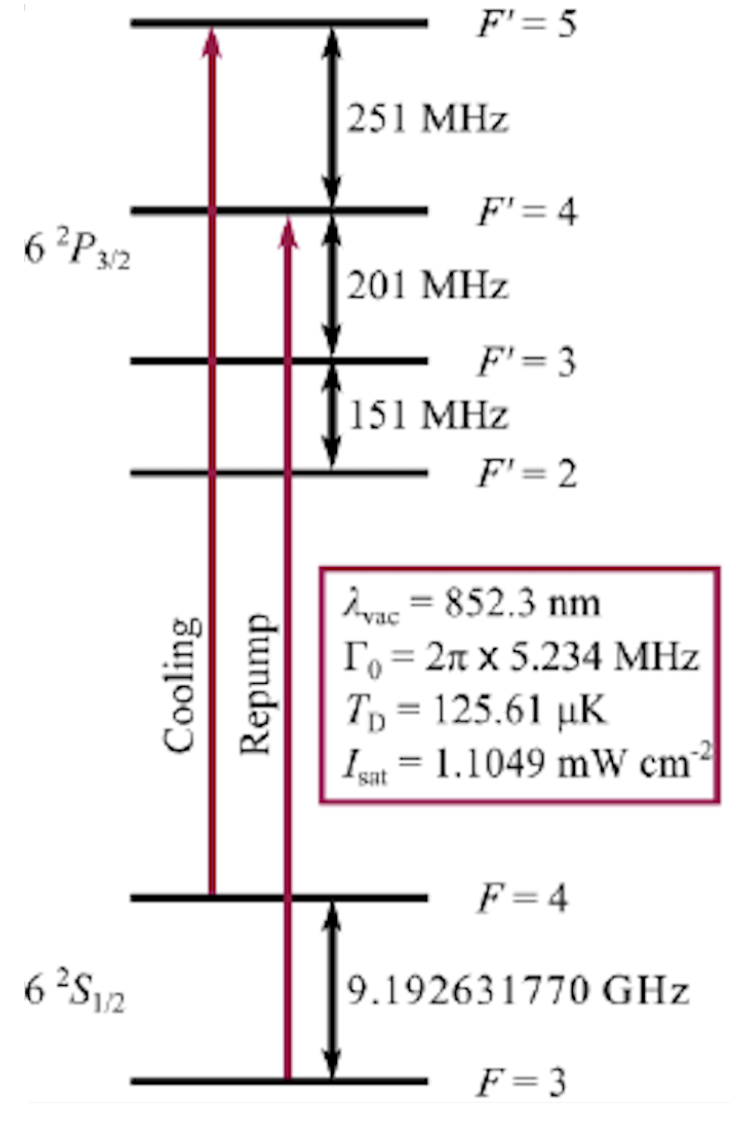
\includegraphics[keepaspectratio,  scale=0.35,  angle=0]
                          {figures/saturated-absorption/Cs_level_diagram_MOT.png}
                          \caption{MOTで用いるCs原子の超微細構造の準位図(参考文献\cite{Cs_level_diagram}から引用)}
                          \label{Cs_level_diagram_MOT}
      \end{minipage}
    \end{tabular}
\end{figure}
\subsection{ECDLによる周波数の制御}
今回の実験で飽和吸収分光に用いるためのレーザーの周波数の制御には外部共振器型半導体レーザー(External Cavity Diode Laser, ECDL)を使用している。ECDLは回折格子の持つ波長選択性を用いて特定のモードの1次回折光をレーザーダイオードに戻すことによりそのモードのゲインを上げ、他のモードのゲインを下げるというものである。この回折格子をピエゾ素子に取り付け、電気的に回折格子の角度を調整できるようにすることで目的の周波数の周辺でレーザーの周波数の挿引を可能にしている。

\begin{figure}[htpb]
  \centering
    \begin{tabular}{c}
      \begin{minipage}{1\hsize}
        \centering
          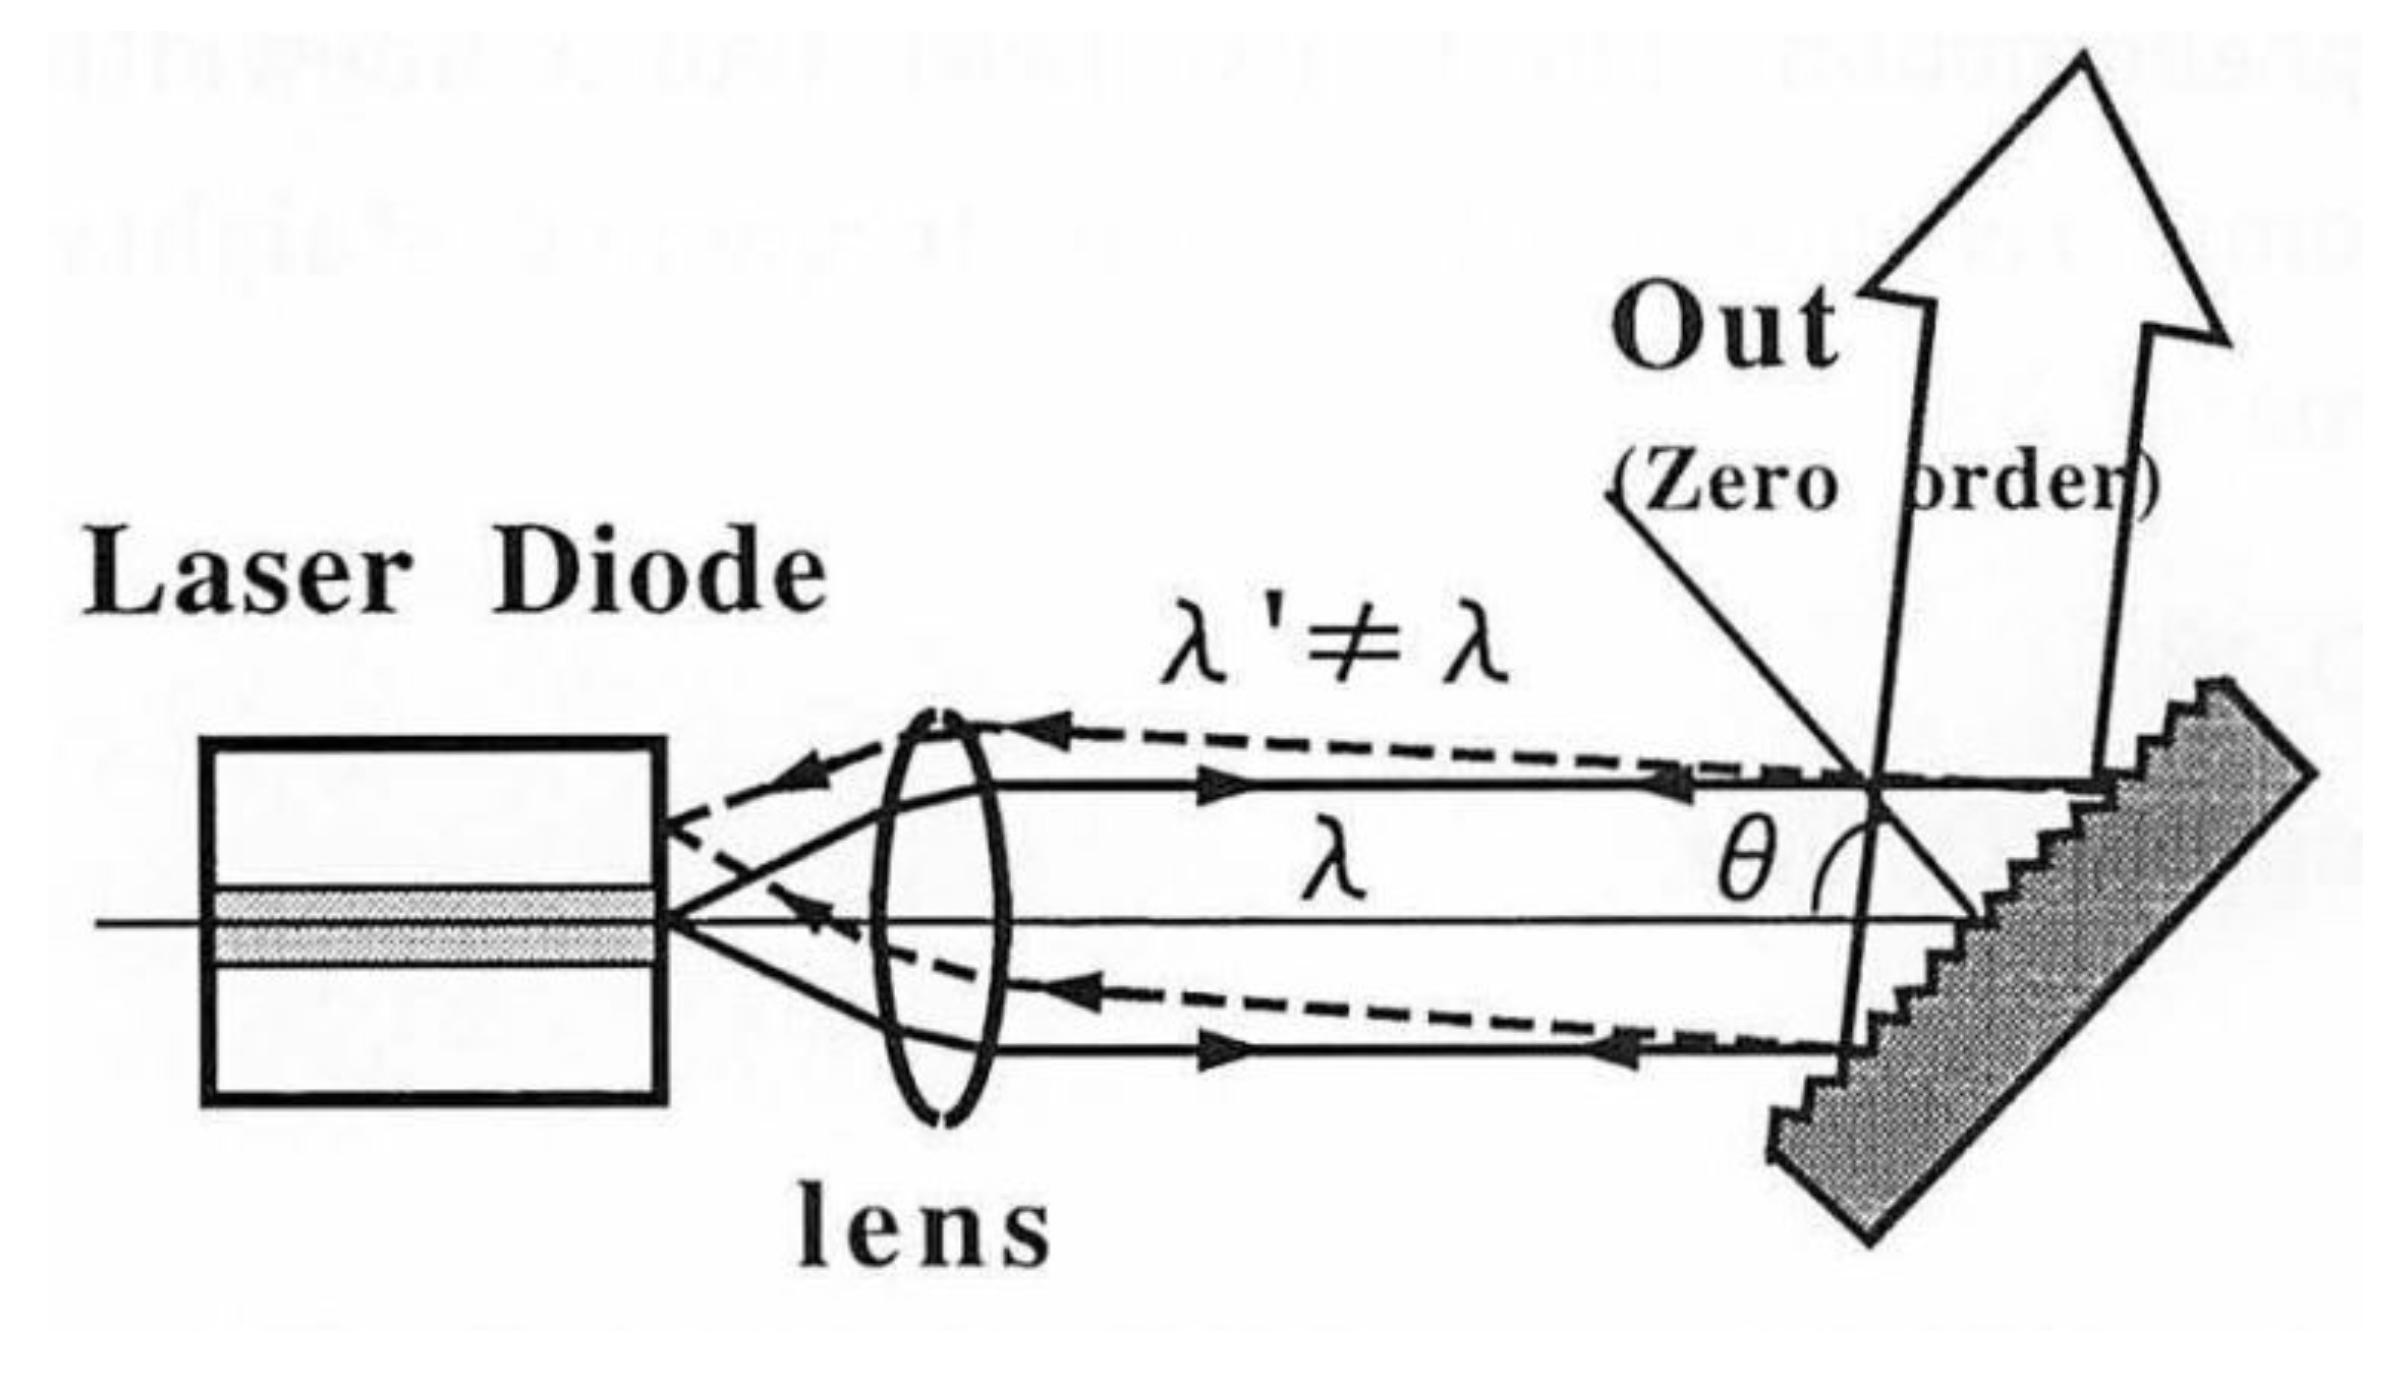
\includegraphics[keepaspectratio,  scale=0.35,  angle=0]
                          {figures/saturated-absorption/ECDL_diagram.png}
                          \caption{ECDLの概略図(参考文献\cite{ECDL}より引用)}
                          \label{ECDL_diagram}
      \end{minipage}
    \end{tabular}
\end{figure}
\subsection{FMサイドバンドロック法}
飽和吸収分光で得られたPDの信号の凹みに周波数をロックするために目的の周波数で正負が逆転するような信号(エラー信号)を生成し、フィードバックをかけることで周波数をロックするという手法を用いる。このエラー信号を生成する手法として用いるのがFMサイドバンドロック法である。この手法では、まず周波数$f_\mathrm{0}$のレーザー光の位相に対して周波数$f_\mathrm{m}$のラジオ周波数の変調を加えることで周波数空間上で元の周波数に対して周波数軸上で両側に二本の$f_\mathrm{0\pm m}$のサイドバンドを立てる。二本のサイドバンドの位相が逆であるため、それぞれのサイドバンドと元の光のヘテロダインビートを取ると、周波数の違いによるCs原子の吸収の差からエラー信号を生成する。
\subsection{今回の飽和吸収分光に用いる光学系}
 今回の実験では、メインレーザーとリポンプレーザーの飽和吸収分光を同一の気体のCs原子が入ったセルを用いて行った。そのため、光学系がやや複雑な形となったので概略図をの二つの図に分けて示した。図\ref{Main_Laser_diagram}はメインレーザーの光学系を示しているが、この光学系の外側に隣接する形で図\ref{repump_diagram}のようにリポンプレーザーの光学系を設置した。
\begin{figure}[htpb]
  \centering
    \begin{tabular}{c}
      \begin{minipage}{1\hsize}
        \centering
          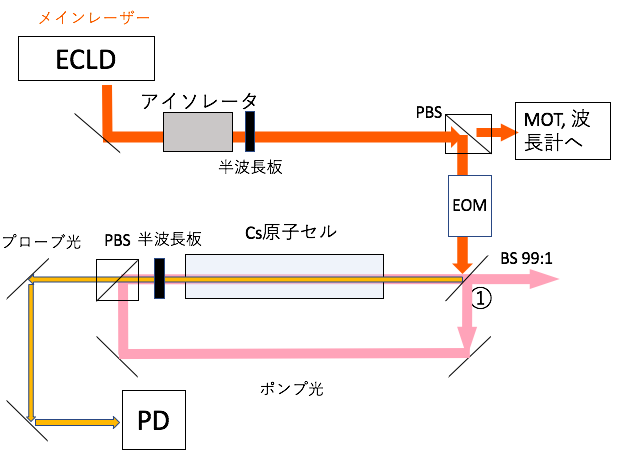
\includegraphics[keepaspectratio,  scale=0.35,  angle=0]
                          {figures/saturated-absorption/Main_Laser_diagram.png}
                          \caption{メインレーザーの光学系}
                          \label{Main_Laser_diagram}
      \end{minipage}\\

      \begin{minipage}{1\hsize}
        \centering
          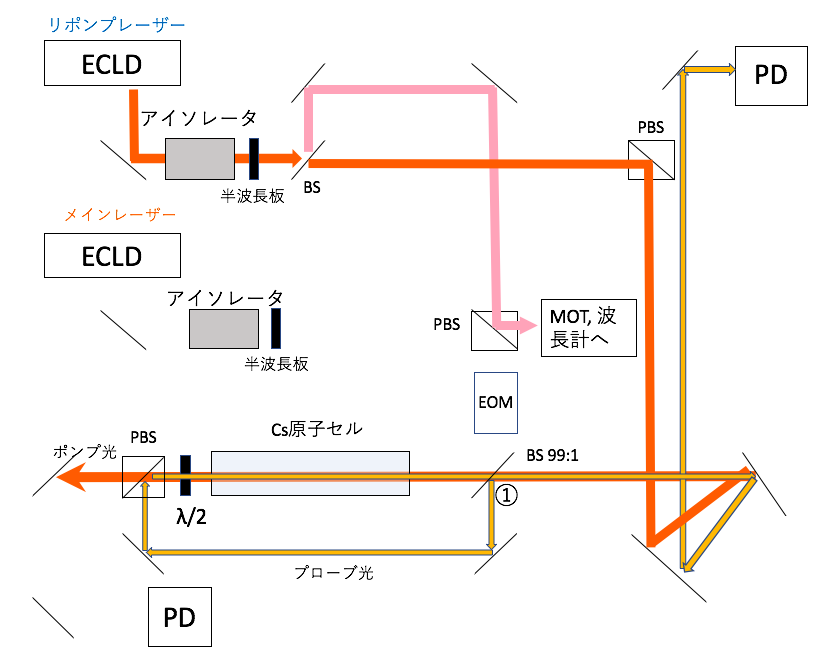
\includegraphics[keepaspectratio,  scale=0.35,  angle=0]
                          {figures/saturated-absorption/repump_diagram.png}
                          \caption{リポンプレーザーの光学系}
                          \label{repump_diagram}
      \end{minipage}
    \end{tabular}
\end{figure}
 どの遷移にロックしているかをのべる。ECDLの仕組み。ピエゾに三角波を入れて周波数の挿引を行なっていることを述べる。エラー信号の得かた。ロック回路。
\section{測定結果}
\subsection{メインレーザーのロック}
メインレーザーの超微細構造を捉えたPDの信号は図\ref{PD_Signal_Main}である。この時のエラーシグナルが図\ref{error_signal_main_all-structure}のようになる。図\ref{main-locking-error}は周波数ロック時のエラー信号である。これらの測定結果から周波数ロック時の線幅を評価することができる。
\begin{figure}[htpb]
  \centering
    \begin{tabular}{c}

      \begin{minipage}{1\hsize}
        \centering
          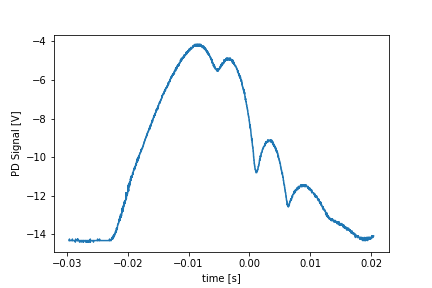
\includegraphics[keepaspectratio,  scale=0.6,  angle=0]
                          {figures/saturated-absorption/PD_Signal_Main.png}
                          \caption{PDで観測されたCs原子の超微細構造(メインレーザー)}
                          \label{PD_Signal_Main}
      \end{minipage}\\

      \begin{minipage}{1\hsize}
        \centering
          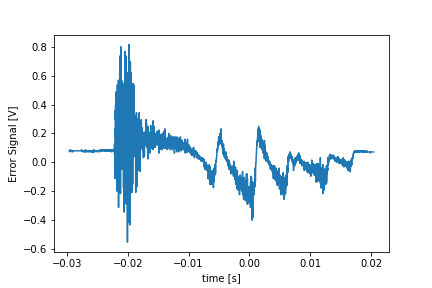
\includegraphics[keepaspectratio,  scale=0.6,  angle=0]
                          {figures/saturated-absorption/error_signal_main_all-structure.png}
                          \caption{図\ref{PD_Signal_Main}の信号のエラー信号}
                          \label{error_signal_main_all-structure}
      \end{minipage}\\

      \begin{minipage}{1\hsize}
        \centering
          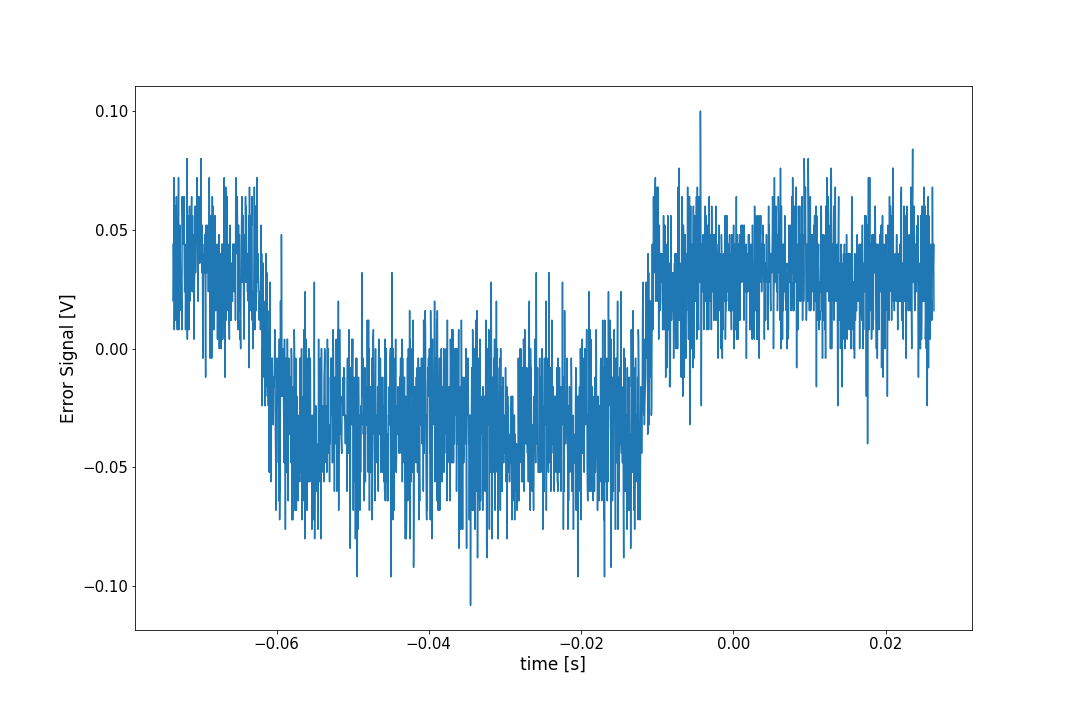
\includegraphics[keepaspectratio,  scale=0.25,  angle=0]
                          {figures/saturated-absorption/main-locking-error.png}
                          \caption{メインレーザーの周波数ロック中のエラー信号}
                          \label{main-locking-error}
      \end{minipage}
    \end{tabular}
\end{figure}

\newpage
\begin{figure}[htpb]
  \centering
    \begin{tabular}{c}
      \begin{minipage}{1\hsize}
        \centering
          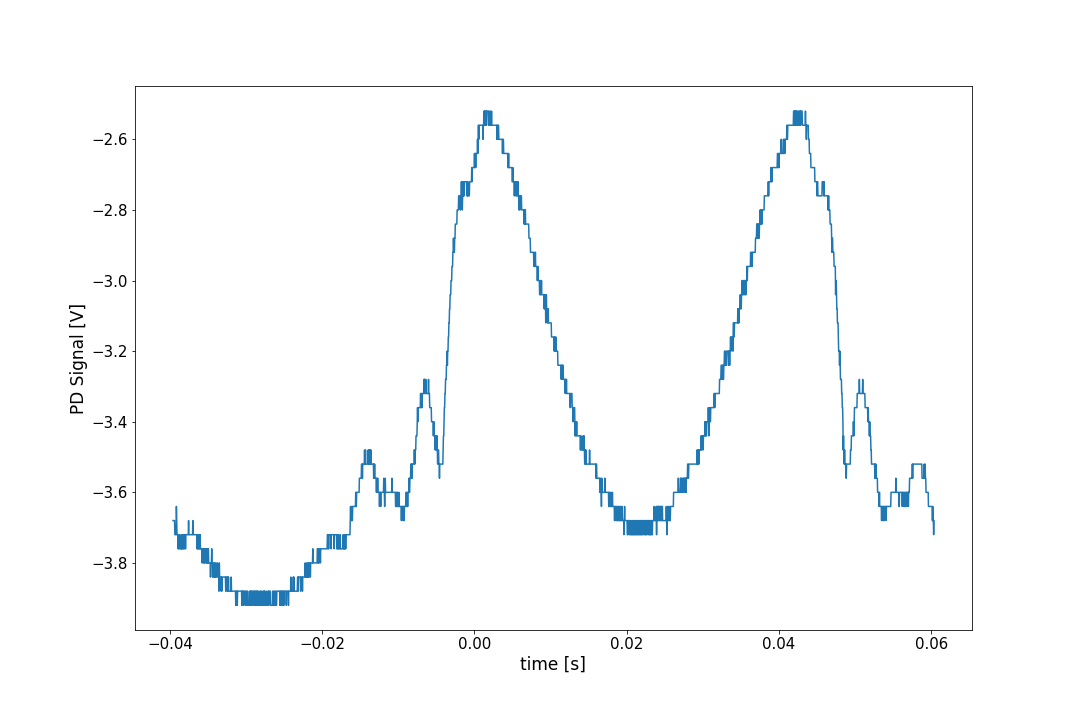
\includegraphics[keepaspectratio,  scale=0.35,  angle=0]
                          {figures/saturated-absorption/Repump_PD_signal.png}
                          \caption{PDで観測されたCs原子の超微細構造(リポンプレーザー)}
                          \label{Repump_PD_signal}
      \end{minipage}
    \end{tabular}
\end{figure}




\newpage
\chapter{光周波数コムのテーパーアンプによる増幅実験}
\section{光周波数コムのテーパーアンプによる増幅}
 二光子励起の励起効率の式(\ref{ResonanceRabi}), (\ref{ExcitationRate})から分かる通り、励起効率はコムの強度の二乗に比例する。そのため、二光子のレーザー冷却を行うに当たり、高効率の二光子励起を実現するためには高強度のレーザーを用意することが非常に重要である。そのため今回の実験では、光周波数コムから得られた光をTAを用いて増幅するという手段を用いる。しかし、通常TAはcwレーザーを増幅するために用いられるため、光周波数コムの増幅に用いた場合にどのような振る舞いを見せるかについての過去の研究は限られており、異なる繰り返し周波数に対してのTAの利得を調べた研究はまだない。今回の実験では繰り返し周波数の異なる光周波数コムに対してTAの増幅の様子を測定した。

\newpage
\section{テーパーアンプのマウンターの組み立て}
 今回の実験では、Cs原子のレーザー冷却に必要なパワーを得るためにTAを用いた。光周波数コムのから$760 \mathrm{nm}$付近の波長と$890 \mathrm{nm}$付近の波長を切り出し増幅した。$890 \mathrm{nm}$側の増幅に用いるTAのチップのマウンターに関しては、設計と組み立てを行った。TAのチップはeagleyard社のEYP-TPA-0915-01500-3006-CMT03-0000を用いた。TAのチップの構造は図\ref{TA_chip_ds}のようになっている。\\
\begin{figure}[htbp]
 \begin{center}
  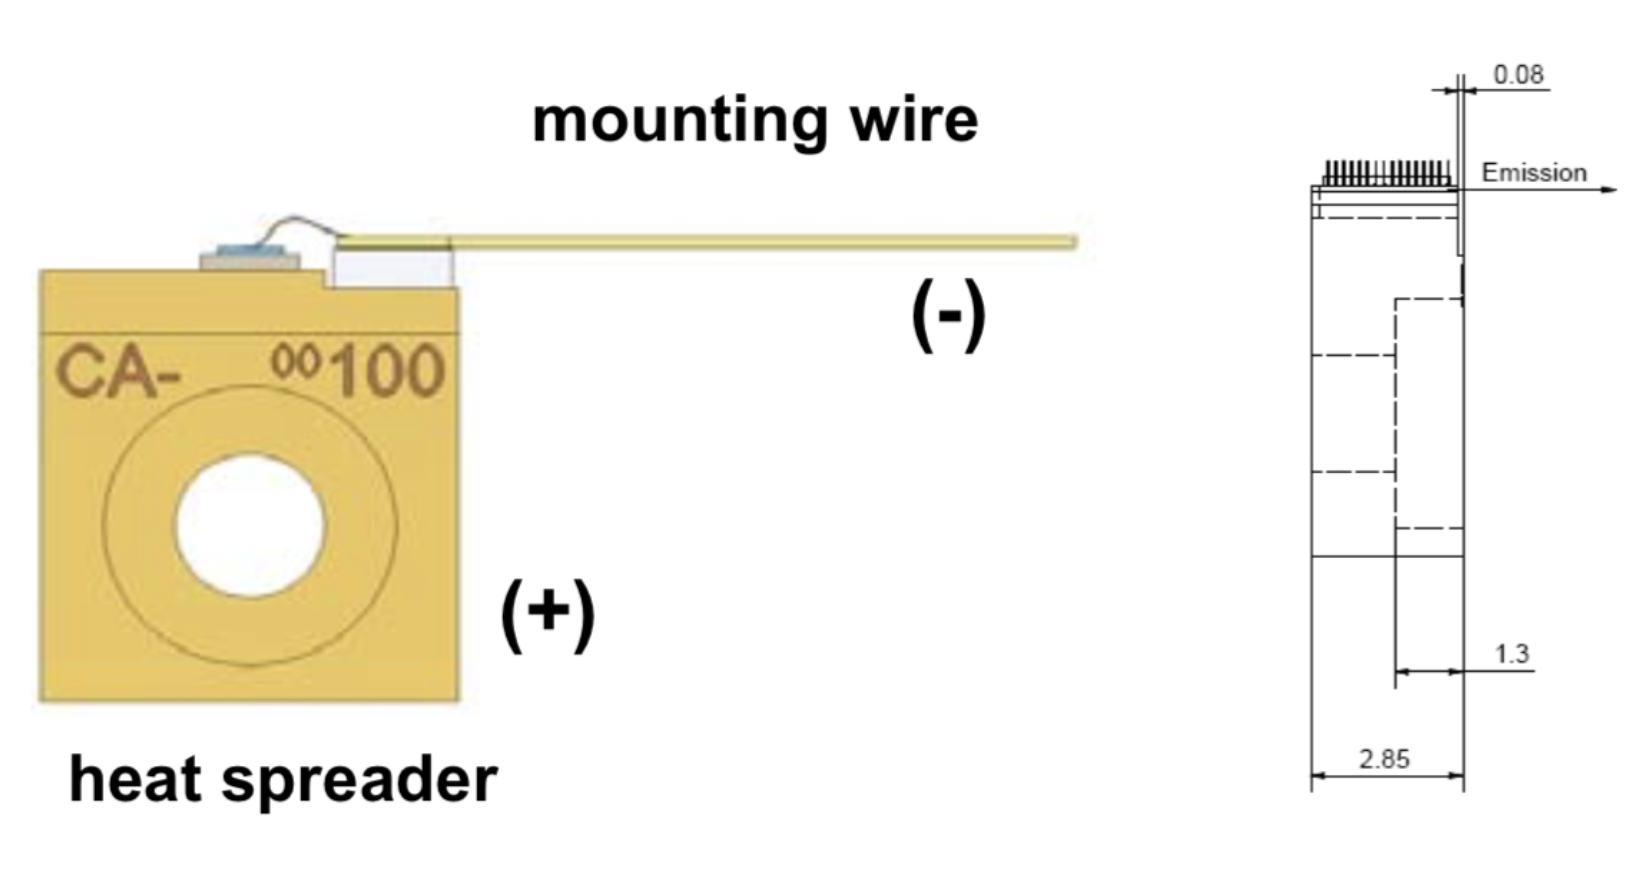
\includegraphics[width=70mm]{figures/chapter4/TA_chip_ds.png}
\end{center}
 \caption{TAチップの構造図(eagleyard社のデータシートから引用)}
 \label{TA_chip_ds}
\end{figure}
 TAチップのマウンターの構造は図\ref{TA_mounter_photo_comments},\ref{TA_mounter_structure}のようになっている。ただし、TAチップの入力光をマスター光、出力光をスレーブ光と呼ぶ。TAチップは銅のブロックにコリメーションレンズ2枚と共に取り付けられており、そこに温度センサーと直流電源からのSMAケーブルが繋がっている。この銅製のブロックをアルミニウム製のブロックを介して光学定盤に固定している。二つのブロックの間にペルチェ素子を挟み、温度を制御している。なお、レンズのマウンターにはアルミニウムを使用している。

\begin{figure}[htpb]
  \centering
    \begin{tabular}{c}

%----- TAチップマウンターの概観 -----

      \begin{minipage}{0.50\hsize}
        \centering
          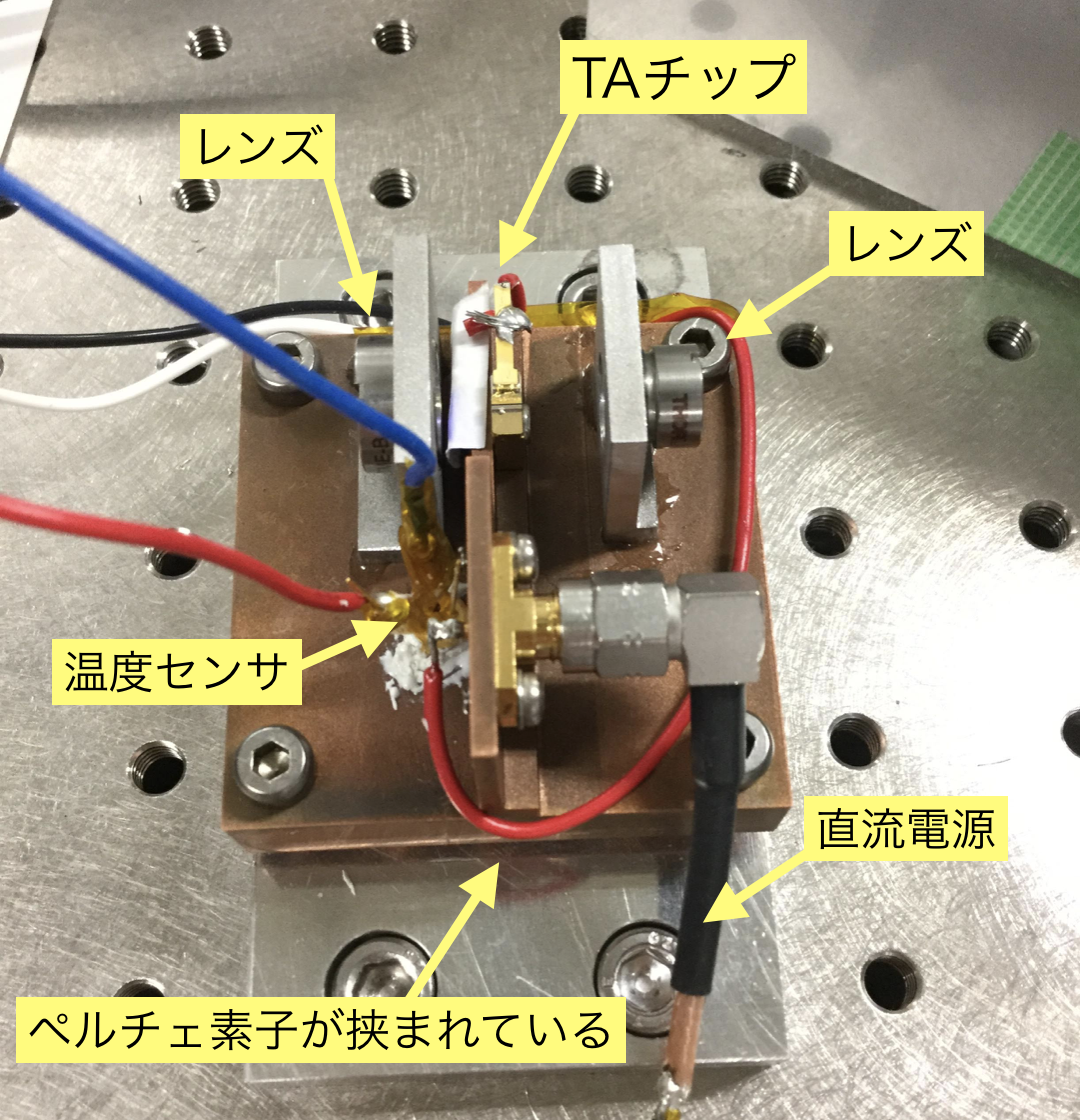
\includegraphics[keepaspectratio,  scale=0.30,  angle=0]
                          {figures/chapter4/TA_mounter_photo_comments.png}
                          \caption{TAチップマウンターの概観}
                          \label{TA_mounter_photo_comments}
      \end{minipage}

%----- TAチップマウンターの構造図 -----

      \begin{minipage}{0.50\hsize}
        \centering
          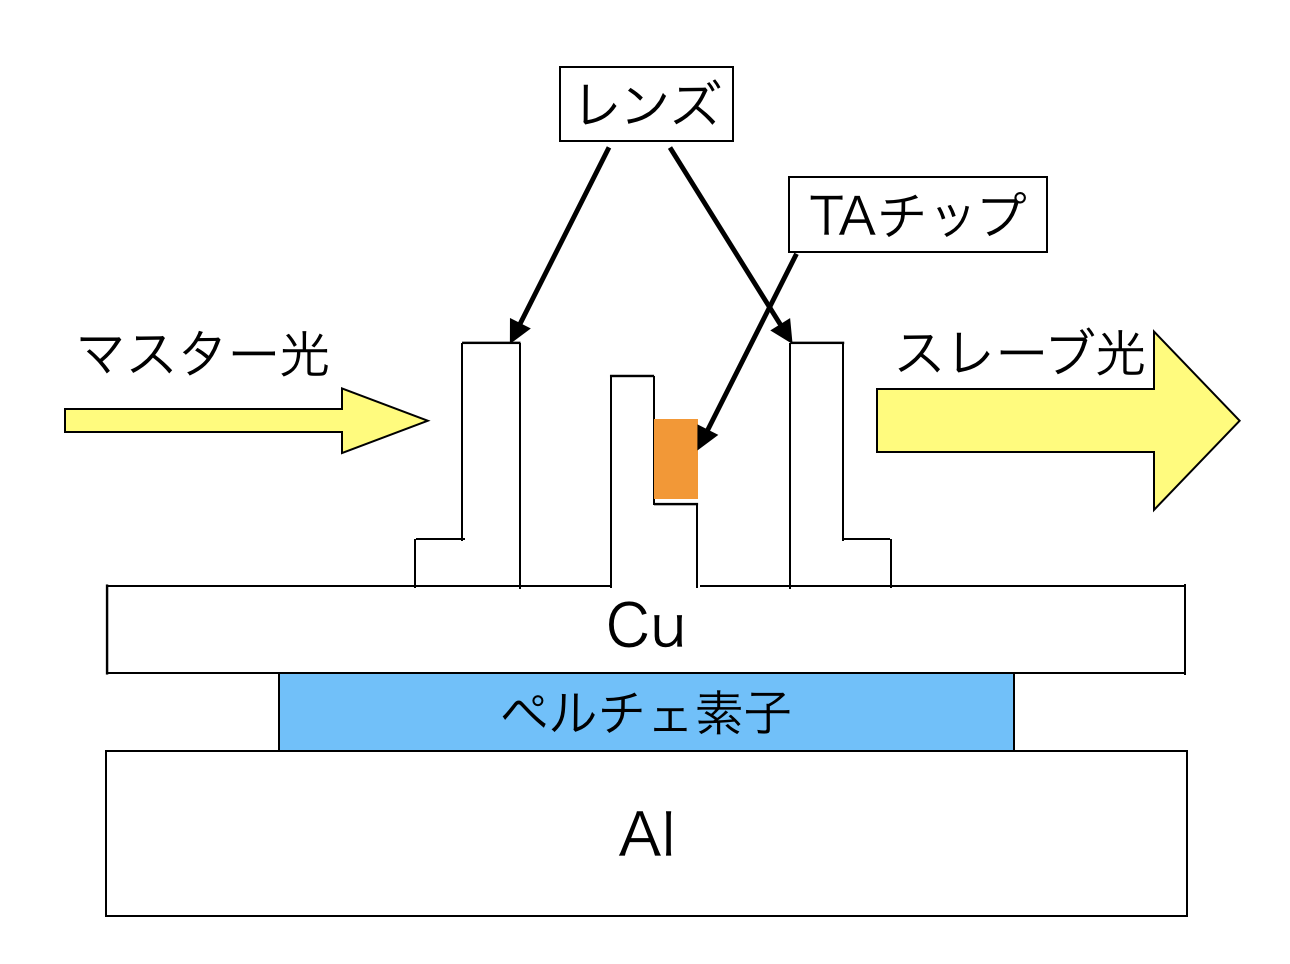
\includegraphics[keepaspectratio,  scale=0.35,  angle=0]
                          {figures/chapter4/TA_mounter_structure.png}
                          \caption{TAチップマウンターの構造図}
                          \label{TA_mounter_structure}
      \end{minipage}

    \end{tabular}
\end{figure}
\newpage
 なお、実際に使用する際には、図\ref{TA_case}のようにアクリルボードでケースを作り使用した。 また、スレーブ光の形状は光の回折の効果から楕円状になっているため、垂直方向のコリメーションを銅ブロック状のレンズで行い、水平方向のコリメーションを追加のシリンドリカルレンズで行う必要がある。\\
\begin{figure}[htbp]
 \begin{center}
  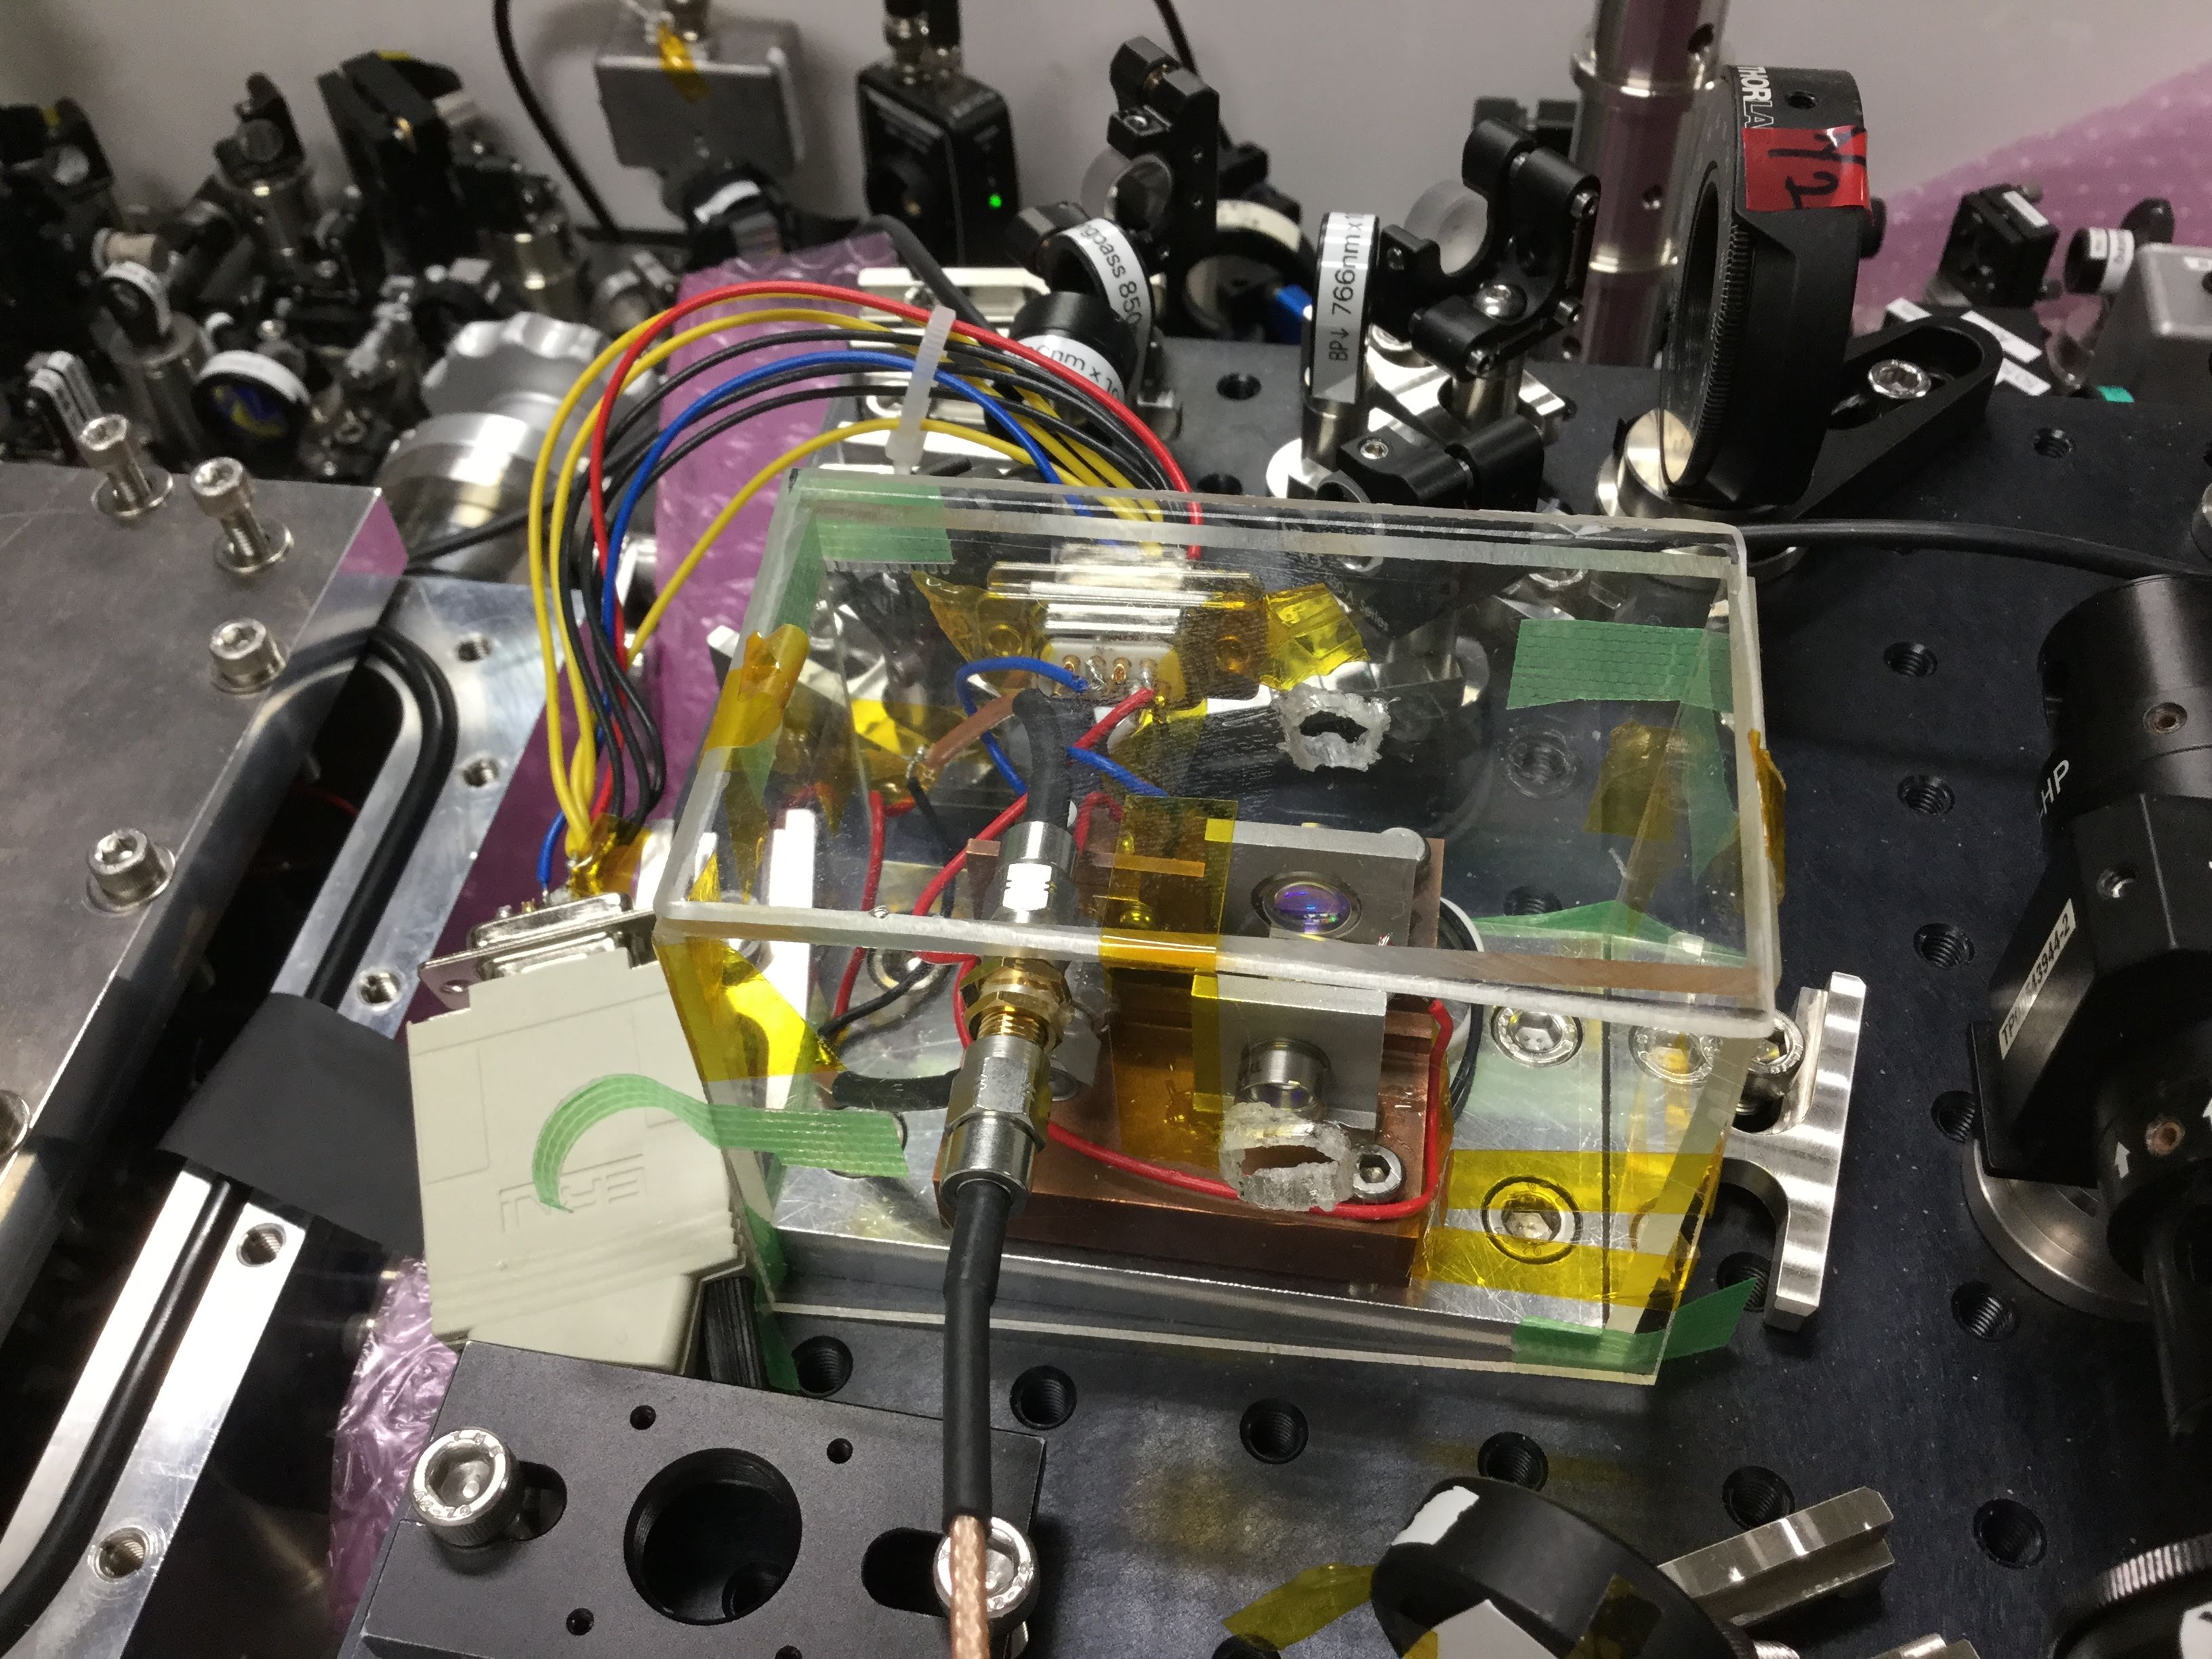
\includegraphics[width=75mm]{figures/chapter4/TA_case.jpg}
\end{center}
 \caption{実際に使用時のTAの様子}
 \label{TA_case}
\end{figure}



\newpage
\section{増幅実験の測定手法}
\subsection{繰り返し周波数の異なるコムでの増幅の比較}
 繰り返し周波数が$120$ MHzと$1.6$ GHzの二台のコムの、$766$ nmを中心波長とする幅$10$ nmのバンドパスフィルター(BPF)を通過した光をTAで増幅させ、マスター光とスレーブ光のパワーを測定した。その際に、BPF通過前のコムのスペクトルと、テーパーアンプの入り口と出口でのコムのスペクトルも測定を行った。その際の光学系は図\ref{760_amp_diagram}, \ref{760_astro_amp_diagram}に示している。繰り返し周波数$120$ MHzのコムを用いた実験ではアイソレータを入れないでTAの実験を行ったところ、TAからの戻り光がコムに光フィードバックをもたらしcw的発振を引き起こすことが観測された。このためアイソレータを使用している。一方で、くり返し周波数が$1.6$ GHzのコムの実験ではアイソレータを使用しなくても、TAからの戻り光がコムの共振器まで戻らずcw的な発振を起こさなかったため、アイソレータは使用しなかった。\\
\subsection{自作のTAでの890nm付近のコムの増幅}
 また、自作したTAで繰り返し周波数が$1.6$ GHzのコムの、$890$ nmを中心波長とする幅$10$ nmのBPFを通過した光を増幅させ、マスター光とスレーブ光のパワーの測定を行った。その際の光学系は図\ref{890_astro_amp_diagram}に示した。
\begin{figure}[htpb]
  \centering
    \begin{tabular}{c}
\begin{comment}
%----- 繰り返し周波数$120$ MHzのコムの$766$ nm付近の光を増幅した際の光学系 -----

      \begin{minipage}{0.5\hsize}
        \centering
          \includegraphics[keepaspectratio,  scale=0.16,  angle=0]
                          {figures/760_amp_experiment_comment.png}
                          \caption{繰り返し周波数$120$ MHzのコムの$766$ nm付近の光を増幅した際の光学系}
                          \label{760_amp_experiment_comment}
      \end{minipage}

%----- 上の写真の概略図 -----
\end{comment}

      \begin{minipage}{0.5\hsize}
        \centering
          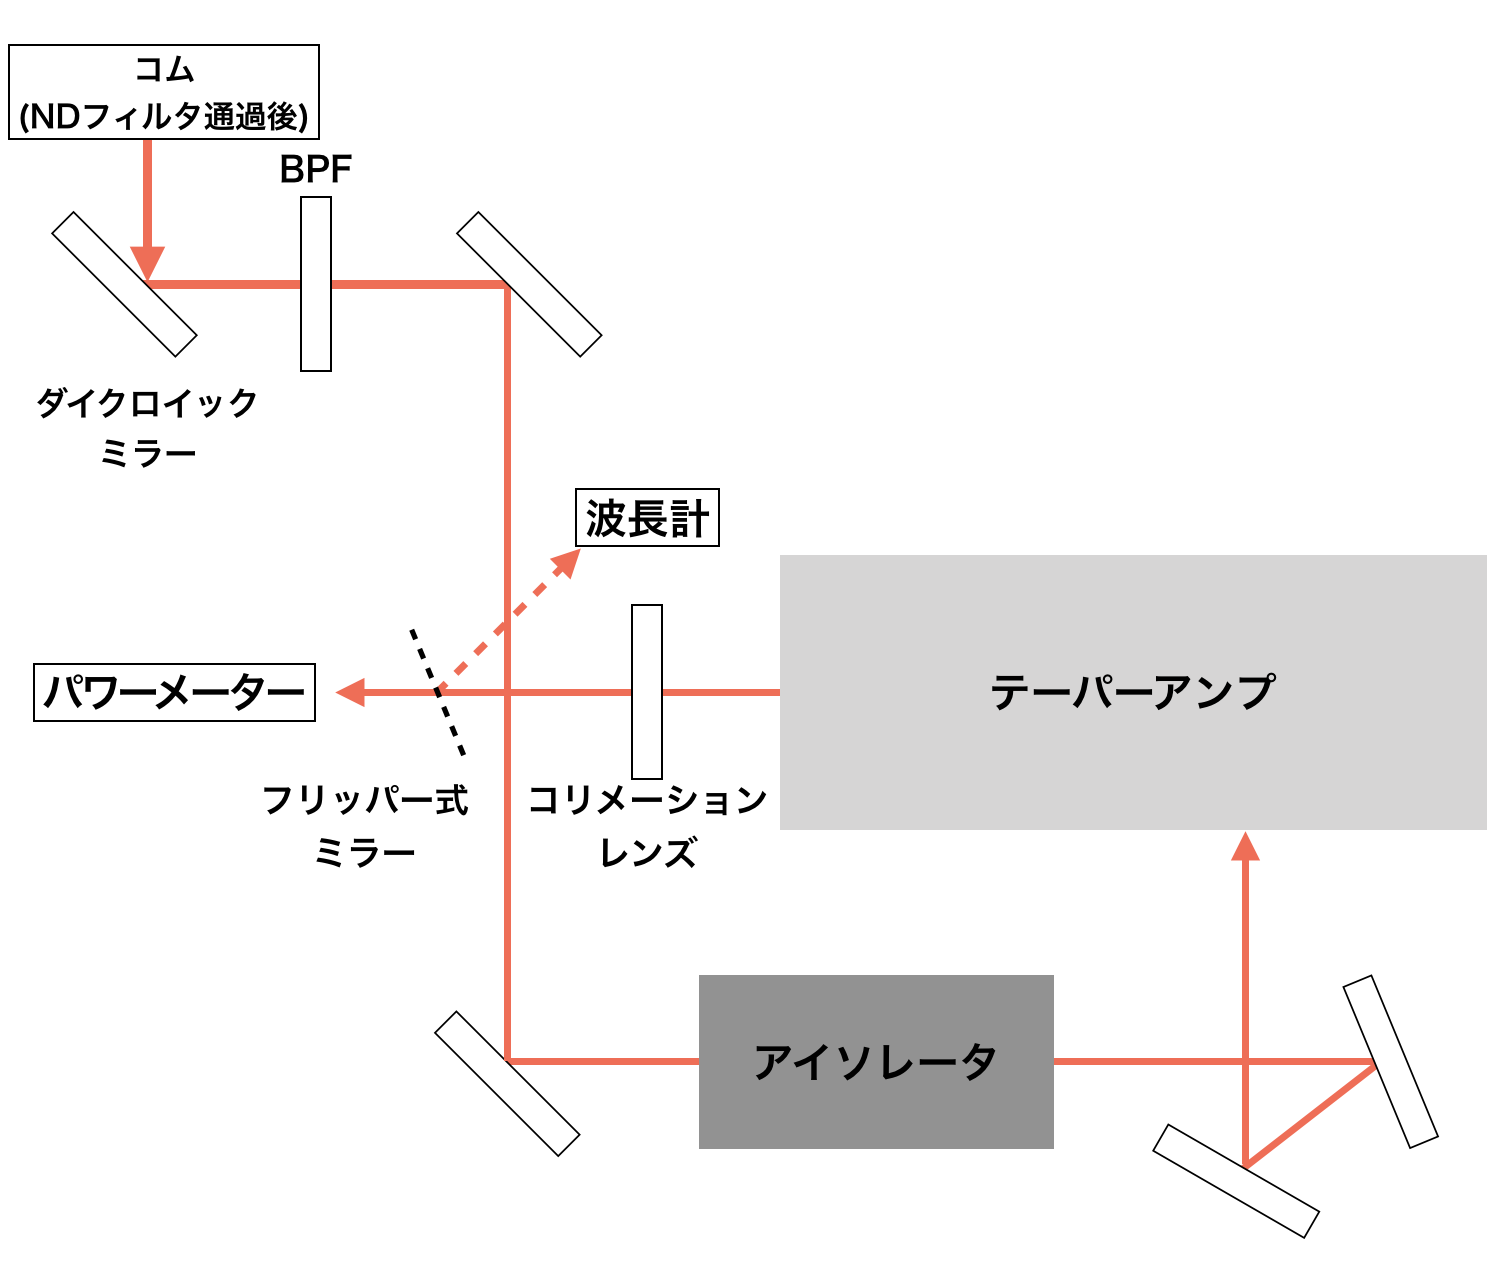
\includegraphics[keepaspectratio,  scale=0.25,  angle=0]
                          {figures/chapter4/760_amp_diagram.png}
                          \caption{繰り返し周波数$120$ MHzのコムの$766$ nm付近の光を増幅した際の光学系\\(アイソレータ有り)}
                          \label{760_amp_diagram}
      \end{minipage}

      \begin{minipage}{0.5\hsize}
        \centering
          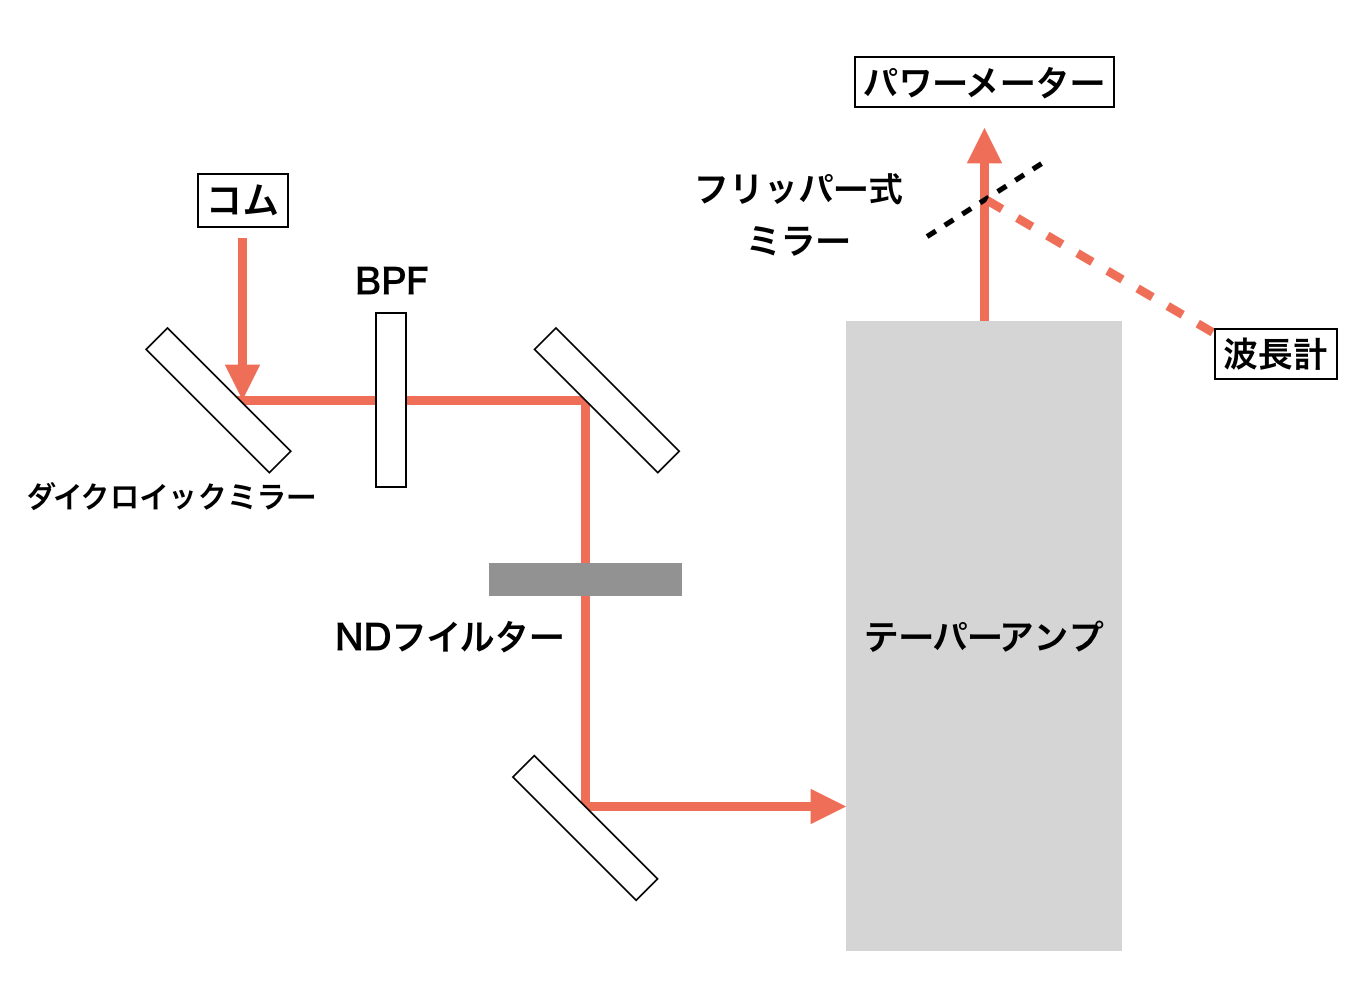
\includegraphics[keepaspectratio,  scale=0.33,  angle=0]
                          {figures/chapter4/760_astro_amp_diagram.png}
                          \caption{繰り返し周波数$1.6$ GHzのコムの$766$ nm付近の光を増幅した際の光学系}
                          \label{760_astro_amp_diagram}
      \end{minipage}\\
      \\

      \begin{minipage}{0.5\hsize}
        \centering
          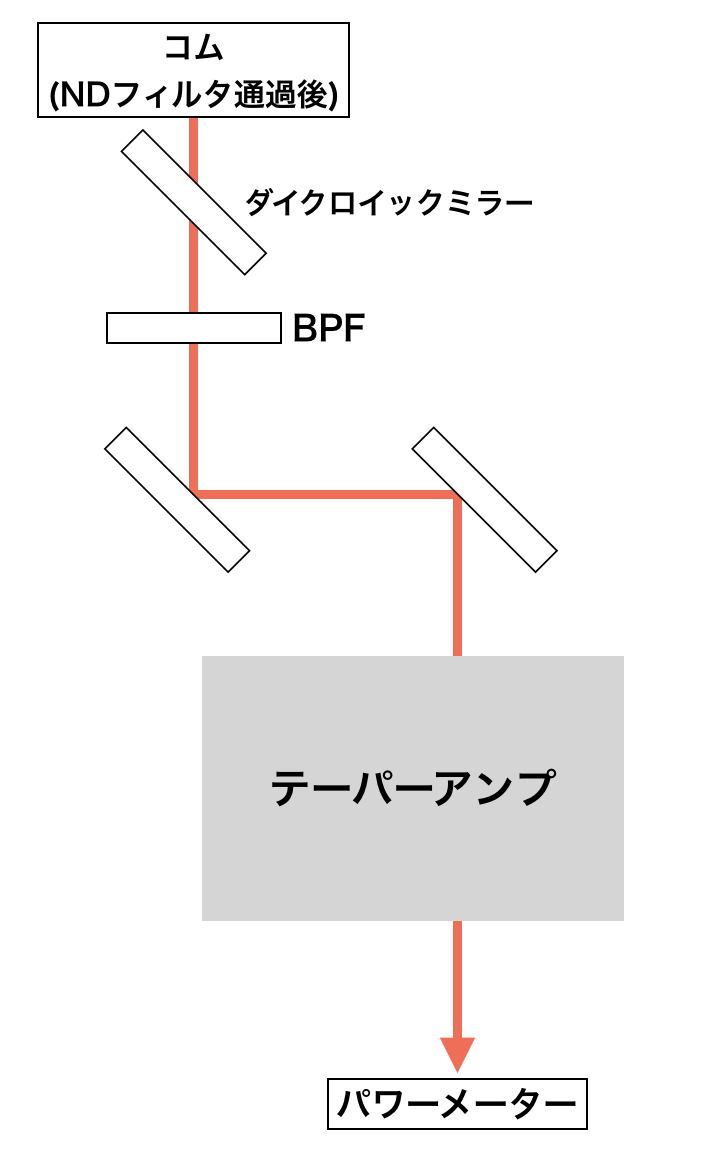
\includegraphics[keepaspectratio,  scale=0.3,  angle=0]
                          {figures/chapter4/890_astro_amp_diagram.png}
                          \caption{繰り返し周波数$1.6$ GHzのコムの$890$ nm付近の光を増幅した際の光学系}
                          \label{890_astro_amp_diagram}
      \end{minipage}

    \end{tabular}
\end{figure}
\newpage
\subsection{ダブルパスによる増幅}
  TAは通常ゲイン領域が細い方からマスター光を入射し、ゲイン領域の広い方からスレーブ光を出力するという使用法をする。しかし、通常の出力側からマスター光を入射し通常の入力側から出た光をミラーで打ち返し再度通常の入力側に光を入射させ、二度ゲイン領域を通過させ増幅するという手法がある。この光学系の配置をダブルパスといい、これに対して通常の配置をシングルパスと呼ぶことがある。ダブルパスでのcwレーザーのTAの増幅の振る舞いについては過去の研究\cite{doi:10.1063/1.3501966}があり、通常cw光でTAを飽和させるには数十ワットのマスター光が必要となるが、ダブルパスの場合だと$200 \mathrm{\mu W}$のマスター光で飽和させることが出来ることが分かっている。また、スペクトルの面でもキャリアの周波数的に幅の広い自然放出が抑えられることが分かっている。このように、ダブルパスによるメリットは多いが光周波数コムの増幅にダブルパスを用いている研究はまだない。そのため今回の実験では,繰り返し周波数$1.6$ GHzの$761$ nmから$771$ nmのコムをダブルパスにより増幅する実験を行った。

 \begin{figure}[htbp]
  \begin{center}
   \includegraphics[width=120mm]{figures/chapter4/doublepass_photo.png}
 \end{center}
  \caption{ダブルパス配置の光学系}
  \label{doublepass_photo}
 \end{figure}

\newpage
\section{測定結果}
\subsection{アイソレータなしの場合のコムのスペクトルの変化}
 図\ref{spectrum_current_MODORI}はマスター光入射時にアイソレータを使用しなかった時の、光周波数コムのキャビティの出力口におけるスペクトラムをTAに印加する電流の大きさを変えつつ分光器で測定したものである。TAの印加電流をあげていくと$770$ nm付近でcw的な発振を起こしていることが分かる。これはTAの入射口から出た自然放出の光が光周波数コムの共振器まで戻り、光フィードバックを起こしているものと考えられる。\\
 そのためマスター光入射時にアイソレータを通過させたところ、スペクトルは図のようになった。このようなcw的な発振は観測されなかった。
\begin{figure}[htbp]
 \begin{center}
  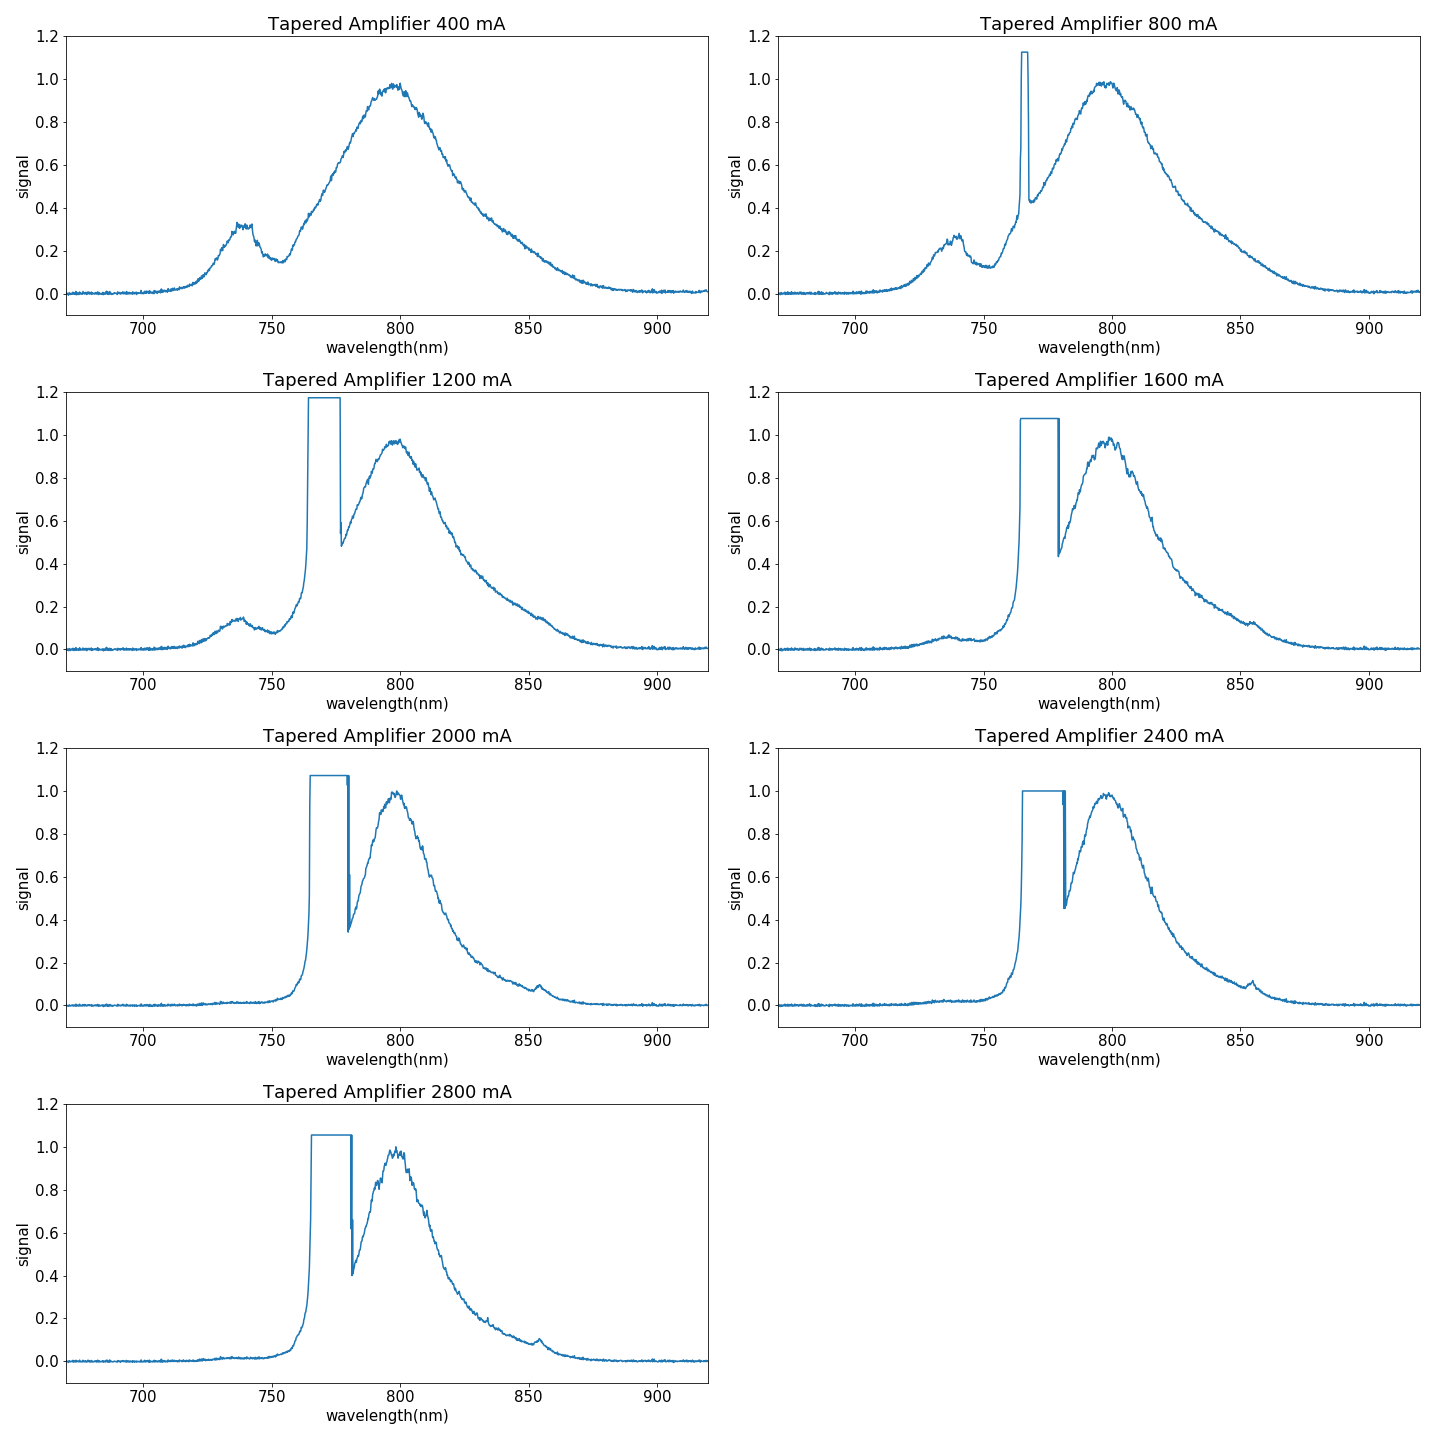
\includegraphics[width=140mm]{figures/chapter4/spectrum_current_MODORI.png}
\end{center}
 \caption{戻り光の影響によるコムのスペクトルの変化}
 \label{spectrum_current_MODORI}
\end{figure}
\newpage
\subsection{繰り返し周波数の異なるコムの増幅}

図\ref{pulse_power-gain-comparison}は766nm側のコムを増幅した際の利得のパルスエネルギー依存性依存性を二つの繰り返し周波数に応じて比較したものである。繰り返し周波数$120 \mathrm{MHz}$の利得をみると、パルスエネルギーの増加に対して利得が低下していく様子がわかる。これは、各パルスに含まれる光子数に対して励起状態にあるキャリア数が足りておらずパルスエネルギーの増加に対して利得を保てていないと考えられる。それに対し、繰り返し周波数$1.6 \mathrm{GHz}$のコムの利得は$120$ MHzのコムの利得を下回っている。これはパルスの時間間隔が$630$ ps程度で短く、十分な反転分布が励起されていないことが原因ではないかと考えられる。\\
 また、スレーブ光強度のマスター光強度依存性を二台のコムで比較すると図\ref{M-S_power-comparison}のようになる。同じマスター光強度で比較すると、繰り返し周波数が$1.6$ GHzのコムのスレーブ光強度が上回っていることがわかる。これは同じ光強度の場合、繰り返し周波数が$120$ MHzのコムでは繰り返し周波数が$1.6$ GHzのコムに比べ一つのパルスに含まれる光子数が多いが、TA内のキャリア数が少ないので誘導放出に使われない光子数が多くなってしまい光が増幅されないことが原因だと考えられる。一方、$1.6$ GHzのコムでは一パルスあたりの光子数が少ないため、無駄になる光子が少なく効率よく増幅することができると考えられる。

\begin{figure}[htpb]
  \centering
    \begin{tabular}{c}

%----- 写真 -----

      \begin{minipage}{0.50\hsize}
        \centering
          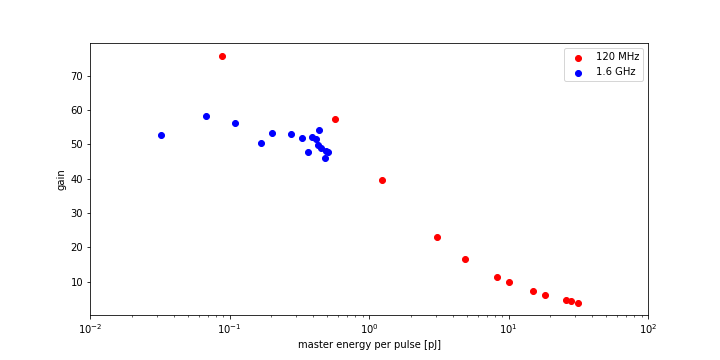
\includegraphics[keepaspectratio,  scale=0.30,  angle=0]
                          {figures/chapter4/pulse_power-gain-comparison.png}
                          \caption{二台のコムにおけるTAの利得のパルスエネルギー依存性の比較}
                          \label{pulse_power-gain-comparison}
      \end{minipage}

%----- PD Signal -----

      \begin{minipage}{0.50\hsize}
        \centering
          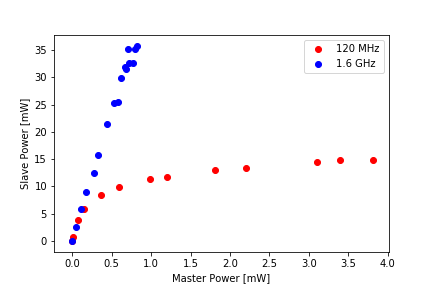
\includegraphics[keepaspectratio,  scale=0.35,  angle=0]
                          {figures/chapter4/M-S_power_comparison.png}
                          \caption{二台のコムにおけるスレーブ光強度のマスター光強度依存性の比較}
                          \label{M-S_power-comparison}
      \end{minipage} \\

      \begin{minipage}{0.50\hsize}
        \centering
          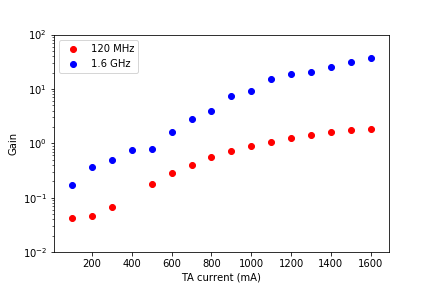
\includegraphics[keepaspectratio,  scale=0.35,  angle=0]
                          {figures/chapter4/TA_cuurent-gain_comparison.png}
                          \caption{二台のコムにおけるTAの利得の印加電流依存性の比較}
                          \label{TA_cuurent-gain_comparison}
      \end{minipage}
    \end{tabular}
\end{figure}
\subsection{繰り返し周波数$1.6$ GHzの$890$ nm付近のコムの増幅}
 繰り返し周波数$1.6$ GHzのコムの$885 \mathrm{nm}から 895 \mathrm{nm}$BPFを通過させた光をTAで増幅した結果を、図\ref{TA_power-current_3A_astro}, \ref{890TPA_power_dependence_0117}に示す。

\begin{figure}[htpb]
  \centering
    \begin{tabular}{c}

%----- 写真 -----

      \begin{minipage}{0.50\hsize}
        \centering
          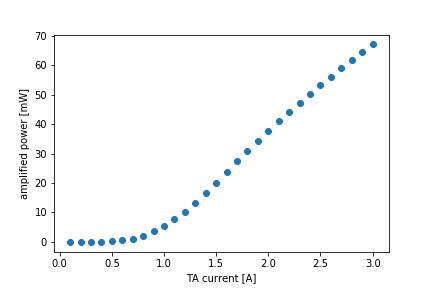
\includegraphics[keepaspectratio,  scale=0.50,  angle=0]
                          {figures/chapter4/TA_power-current_3A_astro.png}
                          \caption{890nm側の繰り返し周波数$1.6$ GHzでのTAのスレーブ光強度の電流依存性}
                          \label{TA_power-current_3A_astro}
      \end{minipage}

%----- PD Signal -----

      \begin{minipage}{0.50\hsize}
        \centering
          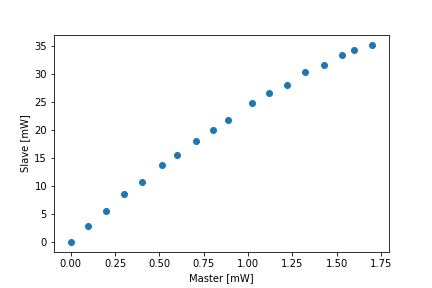
\includegraphics[keepaspectratio,  scale=0.5,  angle=0]
                          {figures/chapter4/890TPA_power_dependence_0117.png}
                          \caption{890nm側の繰り返し周波数$1.6$ GHzでのTAのスレーブ光強度のマスター光強度依存性}
                          \label{890TPA_power_dependence_0117}
      \end{minipage} \\

    \end{tabular}
\end{figure}

\subsection{ダブルパスでの増幅}


\newpage
\begin{figure}[htpb]
  \centering
    \begin{tabular}{c}

      \begin{minipage}{0.70\hsize}
        \centering
          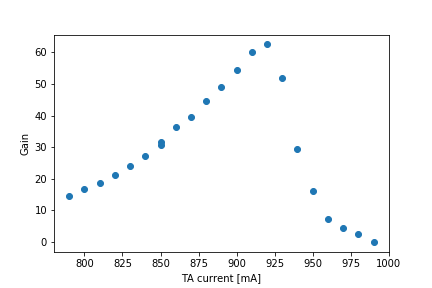
\includegraphics[keepaspectratio,  scale=0.5,  angle=0]
                          {figures/chapter4/double-pass_I-Gain.png}
                          \caption{ダブルパスでの利得の印加電流依存性}
                          \label{double-pass_I-Gain}
      \end{minipage}\\

      \begin{minipage}{1\hsize}
        \centering
          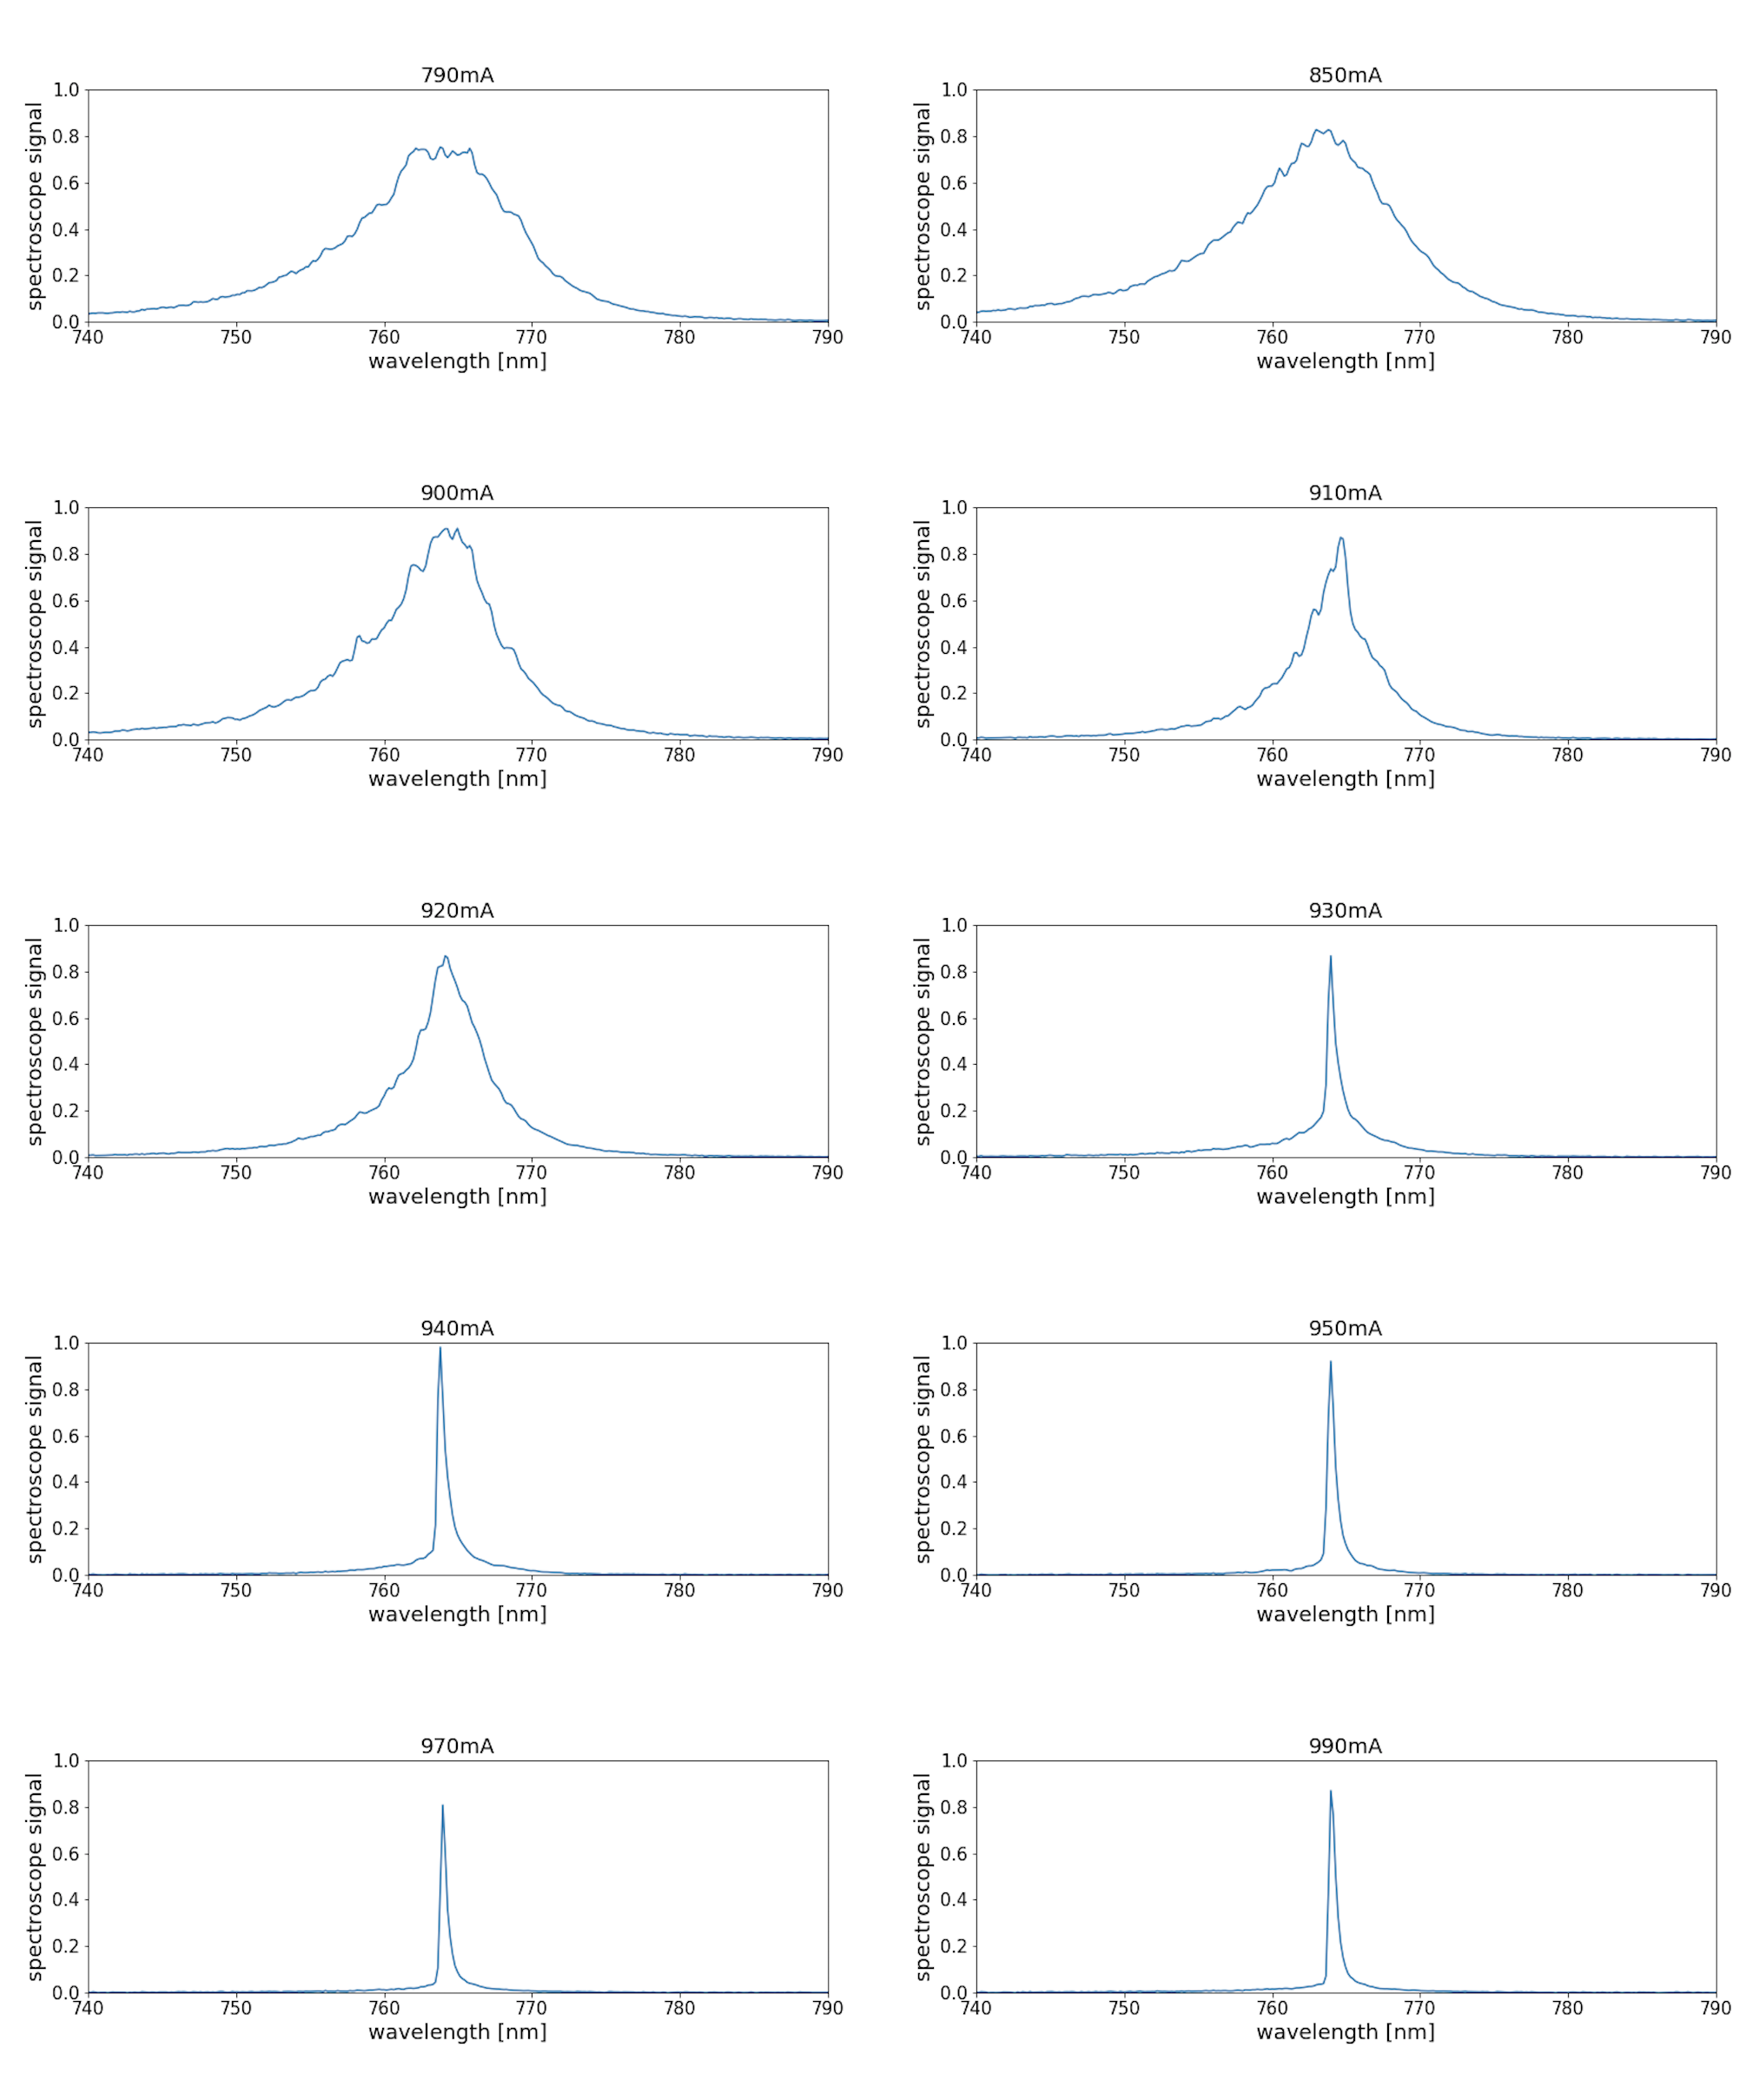
\includegraphics[keepaspectratio,  scale=0.340,  angle=0]
                          {figures/chapter4/double-pass-Slave-Spectrum.png}
                          \caption{ダブルパスでの各印加電流におけるスレーブ光のスペクトル}
                          \label{double-pass_I-Slave}

      \end{minipage}


    \end{tabular}
\end{figure}



\chapter{まとめと展望}






\bibliography{reference}
\end{document}
\end{document}
